\section{Artificial Neural Networks}\label{sec:neural-networks}
\localtableofcontents
Artificial Neural Network (ANN or NN) algorithms for SR are all based on a Convolutional Neural Network (CNN) architecture.
%
We first briefly review ANNs in general, CNNs in particular, powerful architectures called Deep Neural Networks (DNNs), and a powerful training methodology for networks that are generative called Generative Adversarial Networks (GANs).
%
We then proceed to review applications of ANNs to super resolution.
%
\subsection{Basics}
\begin{figure*}
    % MLP
    \centering
    \tikzstyle{inputNode}=[draw,fill=sail,circle,minimum size=10pt,inner sep=2pt]
    \tikzstyle{hiddenNode}=[draw,fill=snowymint,circle,minimum size=10pt,inner sep=2pt]
    \tikzstyle{outputNode}=[draw,fill=plum,circle,minimum size=10pt,inner sep=2pt]
    \tikzstyle{stateTransition}=[-stealth, thick]
    \begin{subfigure}[b]{0.49\textwidth}
        \centering
        \begin{tikzpicture}
            \node[draw,fill=plum, circle,minimum size=25pt,inner sep=0pt] (x) at (0,0) {$\Sigma$ $\sigma$};
            \draw[dashed] (0,-0.43) -- (0,0.43);

            \node[inputNode] (x0) at (-2, 1.5) {$ x_1$};
            \node[inputNode] (x1) at (-2, 0.75) {$ x_2$};
            \node[inputNode] (x2) at (-2, 0) {$ x_3$};
            \node[inputNode] (x3) at (-2, -0.75) {$ x_4$};
            \node[inputNode] (xn) at (-2, -1.95) {$ x_n$};

            \draw[stateTransition] (x0) to[out=0,in=120] node [midway, sloped, above] {$w_1$} (x);
            \draw[stateTransition] (x1) to[out=0,in=150] node [midway, sloped, above] {$w_2$} (x);
            \draw[stateTransition] (x2) to[out=0,in=180] node [midway, sloped, above] {$w_3$} (x);
            \draw[stateTransition] (x3) to[out=0,in=210] node [midway, sloped, above] {$w_4$} (x);
            \draw[stateTransition] (xn) to[out=0,in=240] node [midway, sloped, above] {$w_n$} (x);
            \draw[stateTransition] (x) -- (4,0) node [midway,above] {$z(\mathbf{x}) = \sigma\left(\sum\limits_{i=1}^{n}{w_ix_i} +  b\right)$};
            \node (dots) at (-2, -1.25) {$\vdots$};
        \end{tikzpicture}
        \caption{Single Artificial Neuron function.}\label{fig:singleann}
    \end{subfigure}
    \begin{subfigure}[b]{0.49\textwidth}
        \centering
        \begin{tikzpicture}

            \node[inputNode, thick] (i1) at (6, 0.75) {$x_1$};
            \node[inputNode, thick] (i2) at (6, 0) {$x_2$};
            \node[] (i4) at (6, -0.75) {$\LARGE \vdots$};
            \node[inputNode, thick] (i3) at (6, -1.5) {$x_n$};

            \node[hiddenNode, thick] (h1) at (8, 1.5) {$z_1$};
            \node[hiddenNode, thick] (h2) at (8, 0.75) {$z_2$};
            \node[hiddenNode, thick] (h3) at (8, 0) {$z_3$};
            \node[] (h4) at (8, -0.75) {$\LARGE \vdots$};
            \node[]  at (8, -1.5) {$\LARGE \vdots$};
            \node[hiddenNode, thick] (h5) at (8, -2.25) {$z_m$};

            \node[outputNode, thick] (o2) at (10, 0) {$\Sigma$ $\sigma$};
            \draw[dashed] (10,-0.43) -- (10,0.43);

            \draw[stateTransition] (i1) -- (h1);
            \draw[stateTransition] (i1) -- (h2);
            \draw[stateTransition] (i1) -- (h3);
            \draw[stateTransition] (i1) -- (h5);
            \draw[stateTransition] (i2) -- (h1);
            \draw[stateTransition] (i2) -- (h2);
            \draw[stateTransition] (i2) -- (h3);
            \draw[stateTransition] (i2) -- (h5);
            \draw[stateTransition] (i3) -- (h1);
            \draw[stateTransition] (i3) -- (h2);
            \draw[stateTransition] (i3) -- (h3);
            \draw[stateTransition] (i3) -- (h5);

            \draw[stateTransition] (h1) -- (o2);
            \draw[stateTransition] (h2) -- (o2);
            \draw[stateTransition] (h3) -- (o2);
            \draw[stateTransition] (h5) -- (o2);

            \node[above=of i1, align=center] (l1) {\footnotesize $n$ Neuron \\ \footnotesize Input \\ \footnotesize layer};
            \node[right=1.3em of l1, align=center] (l2) {\footnotesize $m$ Neuron \\ \footnotesize Hidden \\ \footnotesize layer};
            \node[right=2.3em of l2, align=center] (l3) {\footnotesize Output \\ \footnotesize layer};

            \draw[stateTransition] (o2) -- node[midway,above] {$y(\mathbf{x}) = \sigma'\left(\sum\limits_{j=1}^{m}{w'_jz_j} + b'\right)$} (13, 0);
        \end{tikzpicture}
        \caption{Multi-layer ANN.}\label{fig:multiann}
    \end{subfigure}
    \caption{Artificial Neural Network representation.}\label{fig:ann}
\end{figure*}

An ANN is a function specified by compositions of elementary functions called \textit{artificial neurons}\anote{ann} (or simply neurons).
%
Neurons consist of a set of inputs \(\mathbf{x} \coloneqq (x_1, x_2, \dots, x_n)\), a set of parameters called weights \(w_i\), and an textit{activation function} \(\sigma\), which acts as a thresholding mechanism.
%
For example, the simplest function that qualifies as a neuron is a linear function:
\begin{equation}
    z(\mathbf{x}) = w_1 x_1 + w_2 x_2 = \sum_i w_i x_i
    \label{eqn:simpleann}
\end{equation}
where the the activation function is the trivial one i.e., the identity.
%
Common non-trivial, i.e., non-linear, activation functions are the sigmoid function
\begin{equation}
    \operatorname{sig}(x)={\frac {1}{1+e^{-x}}}={\frac {e^{x}}{e^{x}+1}}
\end{equation}
or the hyperbolic tangent function
\begin{equation}
    \tanh x={\frac {\sinh x}{\cosh x}}={\frac {e^{x}-e^{-x}}{e^{x}+e^{-x}}}={\frac {e^{2x}-1}{e^{2x}+1}}
\end{equation}
or the piece-wise defined \textit{rectified linear unit} (\(\operatorname{ReLU}\))
\begin{align}
    \operatorname{ReLU}(x) & \coloneqq \begin{cases}x&{\text{if }}x>0,\\0&{\text{otherwise}}\end{cases} \\
                           & = \max(0, x)
\end{align}
%
Note that eqn.~\eqref{eqn:simpleann} passes through the origin \((0,0,0)\) since it has no constant term; in the parlance of machine learning (ML) the neuron is missing a bias term\anote{bias} \(b\):
\begin{equation}
    z(\mathbf{x}) = \sum_i w_i x_i + b
    \label{eqn:linearregr}
\end{equation}
%
Neurons can be represented as directed graphs where a vertex represent an input or a neuron, and edges represent the weights (see figure~\ref{fig:singleann}).
%
ANNs are then assemblies of neurons grouped into \textit{layers} with the layers composed by applying neurons to outputs from immediately preceding layers.
%
For example the ANN specified in figure~\ref{fig:multiann} represents the function
\begin{equation}
    \begin{split}
        y(\mathbf{x}) &= \sigma' \left( \sum_j w'_j z_j(\mathbf{x}) + b' \right) \\
        &=  \sigma' \left( \sum_{j=1}^m w'_j \sigma\left(\sum_{i=1}^n w_i x_i + b_j\right) + b' \right)
    \end{split}
\end{equation}
%
Layers are categorized as either \textit{hidden layers} or input-ouput layers: those layers that are not input or output layers are hidden layers.

ANNs might seem like a very simple class of functions; for example, Minsky \etal\cite{minsky2017perceptrons} famously proved that ANNs that don't include a non-linear activation functions can't represent \(\operatorname{XOR}\)\anote{xor}. 
%
On the contrary, strikingly, it's the case that ANNs that do include a non-linear activation function fulfill a \textit{universal approximation theorem}\cite{cybenko1989approximation}:
%
given any continuous function \(f\) (on some bounded interval \(I\)) there exists a sequence of ANNs (with at least one hidden layer and employing a non-linear activation function) whose limit approximates\anote{uniformconv} \(f\) to arbitrary precision.
%
A critical component of the universal approximation theorem is finding the correct sequence of ANNs; in the parlance of ML an ANN demands a \textit{learning rule}.
%
In general, ANN learning rules iterate on the the weights \(w_i\) given \(k \gg 1\) \textit{training} pairs of known inputs and ouputs \(\left\{ \bm{x}_k, t_k \right\}\) of \(f\). 
%
The \(\mathbf{x}_k\) are called the \(k\)th \textit{training samples} and \(t_k\) the  \textit{training targets}.
%
The most common such learning rule is a \textit{gradient descent} based rule called the Delta rule\cite{widrow1960adaptive}.
%
It is derived from minimizing the \(L_2\) \textit{loss} with respect to each of the weights using gradient descent:
\begin{equation}
    L(w_1, \dots, w_n) \coloneqq \sum_k \frac{1}{2} (t_k - y(\mathbf{x}_k))^2
    \label{eqn:loss}
\end{equation}
and hence
\begin{equation}
    \pd{L}{w_i} = - \sum_k(t_k-y(\bm{x}_k))\cdot y'\cdot x_{ik}
\end{equation}
where here by \(y' \coloneqq \sigma'\) we mean the derivative of the activation function with respect to its argument and by \(x_{ik}\) we mean the \(i\)th input \(x_i\) of the \(k\)th training sample \(\bm{x}_k\).
%
Hence, by gradient descent the weights \(w_i\) should be adjusted in the opposite direction of \(\pd{L}{w_i}\) and so we have the weight update rule
\begin{equation}
    \Delta w_i \coloneqq \alpha \cdot \sum_k(t_k-y(\mathbf{x}_k))\cdot \sigma'\cdot x_{ik}
    \label{eqn:batchupdate}
\end{equation}
where \(\alpha\) is a small constant called the \textit{learning rate} that controls the rate of convergence of the ANN.

In general computing the partial derivatives \(\pd{L}{w_i}\) for a deep (many layers) and wide (many neurons in each layer) network is onerous.
%
\begin{figure}[!htbp]
    \centering
    \begin{subfigure}[b]{.49\textwidth}
        \centering
        \begin{tikzpicture}[]
            \def\pindist{35pt}
            \def\nodesize{38pt}

            \tikzstyle{every pin edge}=[signal]
            \tikzstyle{annot} = [text width=4em, text centered]

            \node[hiddennode, text width=\nodesize, minimum size=\nodesize,
                pin={[pin edge={latex-}, pin distance=\pindist]above left:$w_1 x_1$},
                pin={[pin edge={latex-}, pin distance=\pindist]below left:$w_2 x_2$},
                pin={[pin edge={-latex}, pin distance=\pindist]right:$y$}
            ] (N1) at (-100pt,0) {$\Sigma\quad \sigma$};
            \draw[dashed] (-100pt,-0.55) -- (-100pt,0.55);
        \end{tikzpicture}
        \caption{Forward Pass.}
    \end{subfigure}
    \vskip\baselineskip
    \begin{subfigure}[b]{.49\textwidth}
        \centering
        \begin{tikzpicture}[]
            \def\pindist{35pt}
            \def\nodesize{38pt}
            \tikzstyle{every pin edge}=[signal]
            \tikzstyle{annot} = [text width=4em, text centered]

            \node[hiddennode, text width=\nodesize, minimum size=\nodesize,
                pin={[pin edge={-latex}, pin distance=\pindist]above left:$\frac{\partial L}{\partial w_1}=\frac{\partial L}{\partial y}\frac{\partial y}{\partial w_1}$},
                pin={[pin edge={-latex}, pin distance=\pindist]below left:$\frac{\partial L}{\partial w_2}=\frac{\partial L}{\partial y}\frac{\partial y}{\partial w_2}$},
                pin={[pin edge={latex-}, pin distance=\pindist]right:$\frac{\partial L}{\partial y}$}
            ] (N2) at (+120pt,0) {$\dif \sigma$};
        \end{tikzpicture}
        \caption{Backwards Pass. Note that \(\pd{L}{y}\) can be reused when computing both \(\pd{L}{w_1}\) and \(\pd{L}{w_2}\).}
    \end{subfigure}
    \caption{Back-propagation computation of derivatives.}\label{fig:backprop}
\end{figure}

To mitigate the effect of this combinatorial explosion of dependencies between the weights Rumelhart \etal\cite{rumelhart1988learning} popularlized a technique called \textit{back-propagation}\anote{backprop} or simply backprop (see figure~\ref{fig:backprop}).
%
Another inefficiency of the Delta rule is that it requires evaluating the ANN on the entire set of samples in order to compute the update \(\Delta w_i\).
%
For large training sets (on the order of millions of samples) this is infeasible due to memory limitations.
%
Stochastic Gradient Descent (SGD) replaces computing the total loss in eqn.~\eqref{eqn:batchupdate} with computing a partial loss called the \textit{batch loss}:
\begin{equation}
    \Delta w_i^t = w_i^t - w_i^{t-1} \coloneqq \alpha \cdot \sum_j (t_j-y(\mathbf{x}_j))\cdot \sigma'\cdot x_{ij}
    \label{eqn:sgd}
\end{equation}
where the sum on the left-hand side is now over a subset of samples called a \textit{batch}.
%
This in effect computes the weight update \(\Delta w_i\) incrementally and saves having to hold all training data in memory concurrently.
%
The disadvantage of using SGD is that the batch loss is a noisy estimate of the total loss; in order to assure convergence one typically trains and retrains ANNs on random shufflings of the training data.
%
Each such training episode is called an \textit{epoch}.
%
% Equation~\eqref{eqn:sgd} is evaluated for each of the \(k\) samples sequentially and therefore saves having to store all training samples in memory.
\subsubsection{Convolutional Neural Networks}
The one-dimensional (1-D) discrete convolution \((f*g)\) of 1-D discrete functions \(f,g\) is defined
\begin{equation}
    (f*g)[n]\coloneqq \sum _{i} f[i]g[n-i]
    \label{eqn:1dconv}
\end{equation}
The convolution of a function \(f\) with a finite sequence of values \(g\) can be interpreted as filtering \(f\) with the filter \(g\); for example convolving a noisy \(f\) with a Heaviside function is effectively low-pass filtering \(f\) (see figure~\ref{fig:convfiltering}).
\begin{figure}
    \centering
    \begin{subfigure}[b]{.49\textwidth}
        \centering
        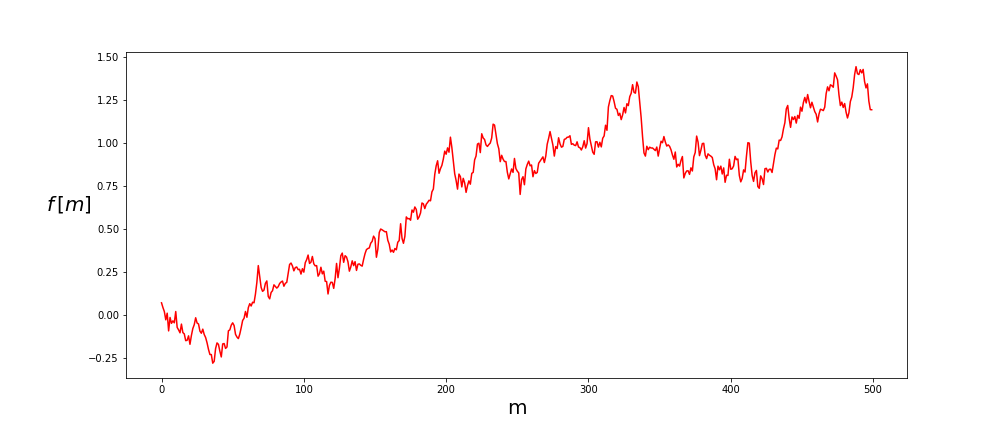
\includegraphics[width=0.95\textwidth]{figures/neural_networks/unsmoothed.png}
        \caption{Noisy function \(f\) (Wiener process sample).}\label{fig:convnoisy}
    \end{subfigure}

    \begin{subfigure}[b]{.49\textwidth}
        \centering
        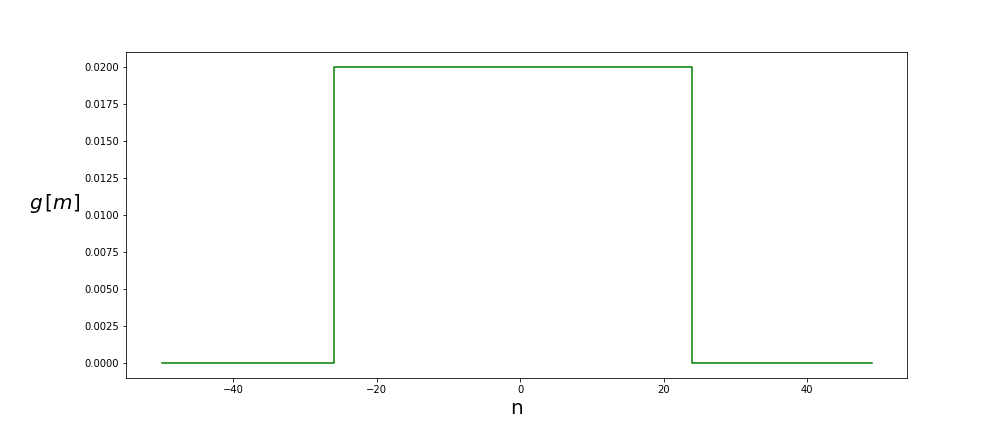
\includegraphics[width=0.95\textwidth]{figures/neural_networks/kernel.png}
        \caption{Heaviside function (low-pass filter \(g\)).}\label{fig:convfilter}
    \end{subfigure}
    \begin{subfigure}[b]{.49\textwidth}
        \centering
        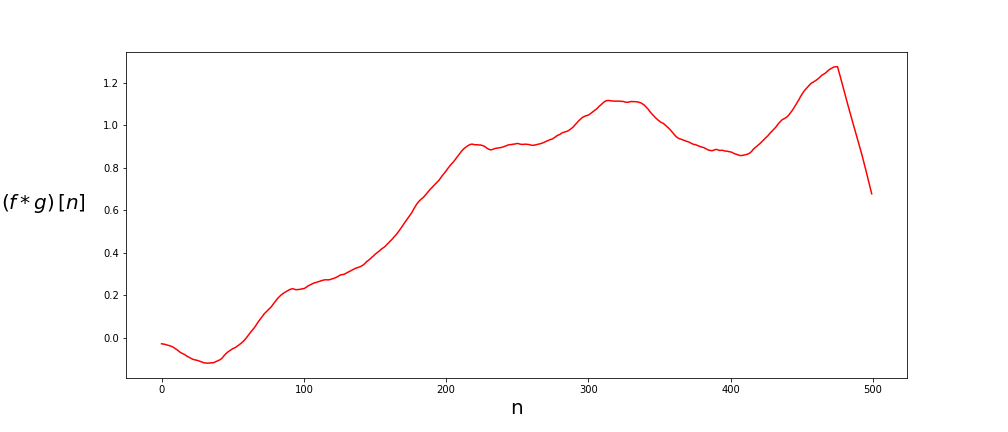
\includegraphics[width=0.95\textwidth]{figures/neural_networks/smoothed.png}
        \caption{Smoothed (low-pass filtered) \(f * g\).}\label{fig:convsmooth}
    \end{subfigure}
    \caption{Convolution as filtering.}\label{fig:convfiltering}
\end{figure}
%
The sequence of values that comprise \(g\) is called the \textit{kernel} of the filter \(g\) and the length of the sequence is called the \textit{bandwidth} of \(g\) (or simply the width).
%
The two-dimensional (2-D) discrete convolution \((f*g)\) of 2-D discrete functions \(f,g\) is defined
\begin{equation}
    (f*g)[n, m]\coloneqq \sum _{i}\sum _{j}f[i, j]g[n-i, m-j]
    \label{eqn:2dconv}
\end{equation}
and can be interpreted in exactly the same way as 1-D convolutions.
%
For 2-D convolutions the kernels are most often square and therefore the kernel dimensions are specified rather than just width (see figure~\ref{fig:2dconv}).
\begin{figure*}
    \centering

    \tikzset{
        inputsquare/.pic={
                \draw[fill=sail] (0,0) rectangle (4,4);
                \draw[black, thick] (0,0) grid (4,4);
                \node at (0.5,0.5) {2};
                \node at (0.5,1.5) {3};
                \node at (0.5,2.5) {0};
                \node at (0.5,3.5) {3};
                \node at (1.5,0.5) {2};
                \node at (1.5,1.5) {1};
                \node at (1.5,2.5) {0};
                \node at (1.5,3.5) {3};
                \node at (2.5,0.5) {3};
                \node at (2.5,1.5) {3};
                \node at (2.5,2.5) {0};
                \node at (2.5,3.5) {2};
                \node at (3.5,0.5) {2};
                \node at (3.5,1.5) {1};
                \node at (3.5,2.5) {1};
                \node at (3.5,3.5) {1};
            },
        pics/filtersquare/.style args={#1/#2/#3/#4}{
                code = {
                        \draw[fill=snowymint] (#1,#2) rectangle (#3,#4);
                        \draw[black, thick] (#1,#2) grid (#3,#4);
                        \node at (#1+0.5,#2+0.5) {0};
                        \node at (#1+0.5,#2+1.5) {2};
                        \node at (#1+0.5,#2+2.5) {0};
                        \node at (#1+1.5,#2+0.5) {0};
                        \node at (#1+1.5,#2+1.5) {2};
                        \node at (#1+1.5,#2+2.5) {0};
                        \node at (#1+2.5,#2+0.5) {1};
                        \node at (#1+2.5,#2+1.5) {0};
                        \node at (#1+2.5,#2+2.5) {2};
                    }},
        pics/outputsquare/.style args={#1/#2/#3/#4}{
                code = {
                        \draw[fill=plum] (0,0) rectangle (2,2);
                        \draw[black, thick] (0,0) grid (2,2);
                        \node at (0.5,0.5) {#3};
                        \node at (0.5,1.5) {#1};
                        \node at (1.5,0.5) {#4};
                        \node at (1.5,1.5) {#2};
                    }}
    }
    \newcommand*{\figwidth}{.25}
    \newcommand*{\figscale}{1}
    \begin{subfigure}[b]{\textwidth}
        \centering
        \begin{tikzpicture}[scale=1,every node/.style={minimum size=1cm},on grid]
            \node (node) at (-0.5,2) {$f = $};
            \pic {inputsquare};
            \begin{scope}[xshift=5cm, yshift=0.5cm]
                \node (node) at (-0.5,1.5) {$g = $};
                \pic {filtersquare=0/0/3/3};
            \end{scope}
            \begin{scope}[xshift=9.5cm, yshift=1cm]
                \node (node) at (-0.75,1) {$f * g = $};
                \pic {outputsquare=7/3/11/12};
            \end{scope}
        \end{tikzpicture}
        \caption{Input \(f\), 2-D \(3 \times 3\) convolution kernel \(g\), and output \(f * g\).}
    \end{subfigure}
    \vskip\baselineskip
    \begin{subfigure}[b]{\textwidth}
        \centering
        \begin{tikzpicture}[scale=\figscale,every node/.style={minimum size=1cm},on grid]
            \begin{scope}[every node/.append style={yslant=0.5,xslant=-0.7},
                    yslant=0.5,xslant=-0.7]

                \pic {inputsquare};
                \coordinate (BL) at (0,1);
                \coordinate (BR) at (3,1);
                \coordinate (TL) at (0,4);
                \coordinate (TR) at (3,4);
            \end{scope}
            \begin{scope}[
                    xshift=-.4,
                    yshift=.4cm,
                    every node/.append style={yslant=0.5,xslant=-0.7,opacity=.4},
                    yslant=0.5,xslant=-0.7]
                \pic{filtersquare=0/1/3/4};

                \coordinate (EBL) at (0,1);
                \coordinate (EBR) at (3,1);
                \coordinate (ETL) at (0,4);
                \coordinate (ETR) at (3,4);

            \end{scope}
            \begin{scope}[xshift=-5, yshift=5cm,
                    every node/.append style={yslant=0.5,xslant=-0.7},
                    yslant=0.5,xslant=-0.7]

                \draw (EBL) -- (0,1) (EBR) -- (1,1)
                (ETL) -- (0,2)    (ETR) -- (1,2);

                \draw (EBL) -- (BL) (EBR) -- (BR)
                (ETL) -- (TL)     (ETR) -- (TR);

                \pic{outputsquare=7/0/0/0};
            \draw[fill=black, opacity=0.3] (0,1) rectangle (1,2);

            \end{scope}
        \end{tikzpicture}
        \begin{tikzpicture}[scale=\figscale,every node/.style={minimum size=1cm},on grid]
            \begin{scope}[every node/.append style={yslant=0.5,xslant=-0.7},
                    yslant=0.5,xslant=-0.7]
                \pic{inputsquare};
                \coordinate (BL) at (1,1);
                \coordinate (BR) at (4,1);
                \coordinate (TL) at (1,4);
                \coordinate (TR) at (4,4);
            \end{scope}
            \begin{scope}[
                    xshift=-.4,
                    yshift=.4cm,
                    every node/.append style={yslant=0.5,xslant=-0.7,opacity=.4},
                    yslant=0.5,xslant=-0.7]

                \pic{filtersquare=1/1/4/4};

                \coordinate (EBL) at (1,1);
                \coordinate (EBR) at (4,1);
                \coordinate (ETL) at (1,4);
                \coordinate (ETR) at (4,4);
            \end{scope}
            \begin{scope}[xshift=-5, yshift=5cm,
                    every node/.append style={yslant=0.5,xslant=-0.7},
                    yslant=0.5,xslant=-0.7]
                \draw (EBL) -- (1,1) (EBR) -- (2,1)
                (ETL) -- (1,2)    (ETR) -- (2,2);
                \draw (EBL) -- (BL) (EBR) -- (BR)
                (ETL) -- (TL)    (ETR) -- (TR);

                \pic{outputsquare=7/3/0/0};
                \draw[fill=black, opacity=0.3] (1,1) rectangle (2,2);

            \end{scope}
        \end{tikzpicture}

        \begin{tikzpicture}[scale=\figscale,every node/.style={minimum size=1cm},on grid]
            \begin{scope}[every node/.append style={yslant=0.5,xslant=-0.7},
                    yslant=0.5,xslant=-0.7]
                \pic{inputsquare};
                \coordinate (BL) at (0,0);
                \coordinate (BR) at (3,0);
                \coordinate (TL) at (0,3);
                \coordinate (TR) at (3,3);
            \end{scope}
            \begin{scope}[
                    xshift=-.4,
                    yshift=.4cm,
                    every node/.append style={yslant=0.5,xslant=-0.7,opacity=.4},
                    yslant=0.5,xslant=-0.7]
                \pic{filtersquare=0/0/3/3};

                \coordinate (EBL) at (0,0);
                \coordinate (EBR) at (3,0);
                \coordinate (ETL) at (0,3);
                \coordinate (ETR) at (3,3);
            \end{scope}
            \begin{scope}[xshift=-5, yshift=5cm,
                    every node/.append style={yslant=0.5,xslant=-0.7},
                    yslant=0.5,xslant=-0.7]
                \draw (EBL) -- (0,0) (EBR) -- (1,0)
                (ETL) -- (0,1)    (ETR) -- (1,1);
                \draw (EBL) -- (BL) (EBR) -- (BR)
                (ETL) -- (TL)    (ETR) -- (TR);

                \pic{outputsquare=7/3/11/0};
                \draw[fill=black, opacity=0.3] (0,0) rectangle
                (1,1);

            \end{scope}
        \end{tikzpicture}
        \begin{tikzpicture}[scale=\figscale,every node/.style={minimum size=1cm},on grid]
            \begin{scope}[every node/.append style={yslant=0.5,xslant=-0.7},
                    yslant=0.5,xslant=-0.7]
                \pic{inputsquare};

                \coordinate (BL) at (1,0);
                \coordinate (BR) at (4,0);
                \coordinate (TL) at (1,3);
                \coordinate (TR) at (4,3);
            \end{scope}
            \begin{scope}[
                    xshift=-.4,
                    yshift=.4cm,
                    every node/.append style={yslant=0.5,xslant=-0.7,opacity=.4},
                    yslant=0.5,xslant=-0.7]
                \pic{filtersquare=1/0/4/3};
                \coordinate (EBL) at (1,0);
                \coordinate (EBR) at (4,0);
                \coordinate (ETL) at (1,3);
                \coordinate (ETR) at (4,3);
            \end{scope}
            \begin{scope}[xshift=-5, yshift=5cm,
                    every node/.append style={yslant=0.5,xslant=-0.7},
                    yslant=0.5,xslant=-0.7]
                \draw (EBL) -- (1,0) (EBR) -- (2,0)
                (ETL) -- (1,1)    (ETR) -- (2,1);
                \draw (EBL) -- (BL) (EBR) -- (BR)
                (ETL) -- (TL)    (ETR) -- (TR);
                \pic{outputsquare=7/3/11/12};
                \draw[fill=black, opacity=0.3] (1,0) rectangle (2,1);

            \end{scope}
        \end{tikzpicture}
        \caption{Evaluation of convolution.}\label{fig:2dconviter}
    \end{subfigure}
    \caption{2-D convolution.}\label{fig:2dconv}
\end{figure*}

Notice that eqns.~\eqref{eqn:1dconv} and~\eqref{eqn:2dconv} are completely linear in their inputs \(f[i]\) (\(f[i,j]\)) with weights \(w_i = g[n-i]\) (\(w_{ij} = g[n-i, m-j]\)) and hence naturally constitute a neuron (layer of neurons); a \textit{convolution layer} in a multi-layer ANN is either eqn.~\eqref{eqn:1dconv} or eqn.~\eqref{eqn:2dconv} with kernel values being iteratively updated by the learning rule.
%
Hence, a CNN is an ANN with one or more convolution layers; CNNs are particularly effective for tasks that operate on images (since image patches have more semantic signficance than image slices).
%
In practice multiple filters are applied to the same input and then stacked to produce a higher-dimensional output (see figure~\ref{fig:multconvs}), each dimension of which is called a \textit{feature map}.
\begin{figure}[!htbp]
    \centering
    \begin{tikzpicture}[scale=.35,every node/.style={minimum size=1cm}, on grid]
        \begin{scope}[]
            \node (node) at (-1.5,2) {$f = $};
            \draw[fill=sail,thick]
            (0,0) grid (4,4) rectangle (0,0);
        \end{scope}

        \foreach \x [count=\i] in {-7,0,7} {%
                \begin{scope}[xshift=\x cm,yshift=8cm]
                    \begin{scope}[xshift=0.5cm,yshift=0.5cm]
                        \node (node) at (-1.5,1.5) {$g_\i = $};
                        \draw[fill=snowymint] (0,0) rectangle (3,3);
                        \draw[black, thick] (0,0) grid (3,3);
                    \end{scope}
                \end{scope}
                \begin{scope}[xshift=\x cm,yshift=16cm]
                    \begin{scope}[xshift=1cm]
                        \node (node) at (-2.5,1) {$f * g_\i = $};
                        \draw[fill=plum] (0,0) rectangle (2,2);
                        \draw[black, thick] (0,0) grid (2,2);
                    \end{scope}
                \end{scope}
            }
        \begin{scope}[xshift=1cm,yshift=24cm]
            \node (node) at (-2,1) {$f' = $};
            \foreach \s in {-0.5,0, 0.5} {%
                    \begin{scope}[xshift=\s cm,yshift=\s cm]
                        \draw[fill=plum] (0,0) rectangle (2,2);
                        \draw[black, thick] (0,0) grid (2,2);
                    \end{scope}
                }
        \end{scope}
        \draw[thick] (-0.5,3.5)   -- (-5,8);
        \draw[thick] (2,4.5)      -- (2,8) ;
        \draw[thick] (4.5,3.5)    -- (9,8) ;

        \draw[thick] (-5,12) -- (-5,15.5);
        \draw[thick] (2,12) -- (2,15.5)  ;
        \draw[thick] (9,12) -- (9,15.5)  ;

        \draw[thick] (-5,18.5) --(-0.125,23.5);
        \draw[thick] (2,18.5) -- (2,23)   ;
        \draw[thick] (9,18.5) -- (4.125,23.5) ;
    \end{tikzpicture}
    \caption{A convolution layer consisting of three distinct \(3\times 3\) filters.}\label{fig:multconvs}
\end{figure}
%
Depending on whether the CNN is being employed to solve a generative task or a classification task the activation function might be either a \(\operatorname{ReLU}\) (applied element-wise to the output of the convolution layer) or a \textit{max-pooling} filter:
\begin{multline}
    \operatorname{max-pool}(f,g)[n, m]\coloneqq\\ \max_{i,j}\left[ f[i, j]g[n-i, m-j] \right]
    \label{eqn:2dpool}
\end{multline}
There are many other convolution operators (e.g., strided, dilated, transposed) that are beyond the scope of this survey\cite{dumoulin2016guide}.

\subsubsection{Deep Neural Networks}\label{subsubsec:dnns}

%
Deep Neural Networks (DNNs) are ANNs that have multiple layers and many neurons in each layer.
%
Intuitively the advantage of deep networks (over shallow networks) is they learn\anote{learn} hierarchies of concepts (called \textit{features}); for example in face recognition tasks, layers proximal to the input layer learn to recognize elementary features such as edges, layers distal to the input layer learn abstractions such as arrangements of features that comprise eyes or noses, and layers even more distal to the input layer learn entire faces.

Training DNNs presents many challenges; due to their depth they suffer from issues such as \textit{vanishing gradients} and \textit{overfitting}.
%
Vanishing gradients is an all but complete cessation of substantive updates to weights; consider the partial derivative of the activation function \(\sigma'\) in eqn.~\eqref{eqn:batchupdate}.
%
Notice that if \(\abs{\sigma'} \ll 1\) then \(\Delta w_i\) will be very small.
%
This occurs for a single neuron when the input \textit{saturates} the activation function; for example for \(\operatorname{sig}\) this happens when \(\abs{x} > 5\) because the gradient \(\sigma'\) is very small (see figure~\ref{fig:activs}).
\begin{figure}
    \centering
    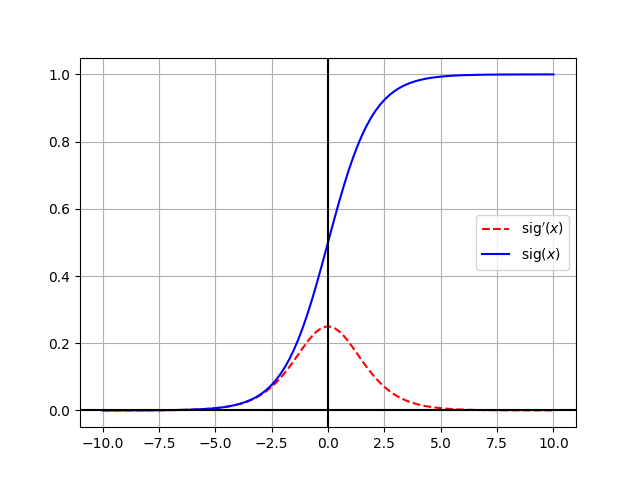
\includegraphics[width=\linewidth]{figures/neural_networks/activation_grads.png}
    \caption[]{Sigmoid activation gradients. Note that for \(\abs{x} > 5\) the gradient is almost 0.}\label{eqn:activs}
\end{figure}
%
For multi-layer ANNs, such as DNNs, even if no single neuron saturates the activation function,
due to the chain rule, weight updates for layers near the input potentially have products of very many factors that are less than one.
%
Overfitting can be interpreted as memorization of the training samples; since the optimization (eqn.~\eqref{eqn:loss}) that leads to the Delta rule only measures \(\abs{t_k - y(\mathbf{x}_k)}\) DNNs can simply learn weights that encode responses to many (or most) of the training samples (since DNNs have so many weight parameters\anote{largeparams}).

Deep Learning is a collection of techniques that make training Deep Neural Networks (DNNs) tractable.
%
\begin{figure}
    \centering
    \begin{subfigure}[c]{0.49\textwidth}
        \centering
        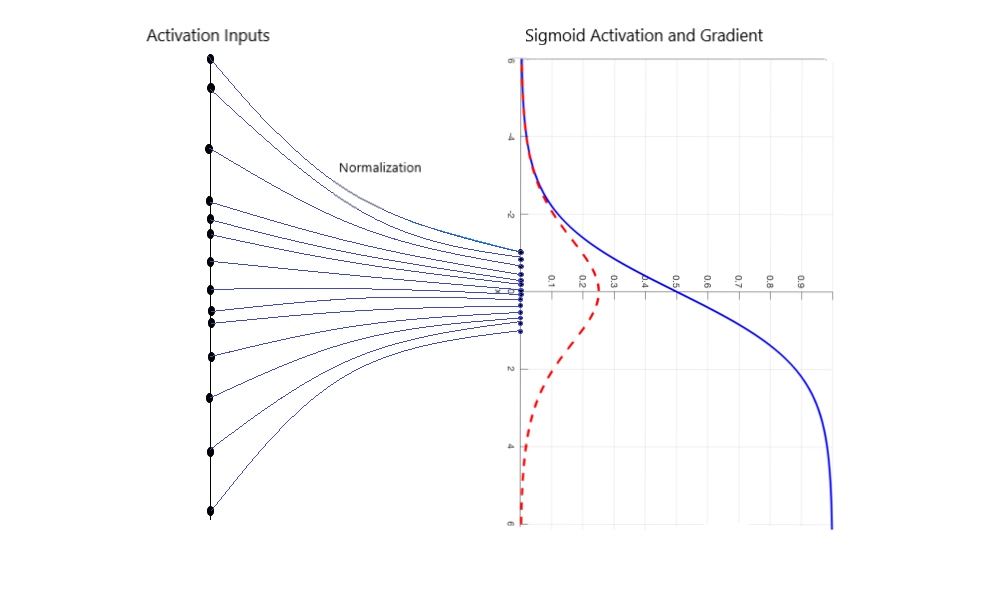
\includegraphics[width=\textwidth, trim=145 50 145 0, clip]{figures/neural_networks/batch_norm.png}
        \caption[]{Batch normalization's effect, for a single neuron, on inputs to a Sigmoid activation function.}\label{fig:batchnorm1}
    \end{subfigure}

    \begin{subfigure}[b]{0.49\textwidth}
        \centering
        \begin{tikzpicture}[
            start chain=going below, node distance=12pt,
            point/.append style={on chain, join=by {signal}},
            layer/.append style={on chain, join=by {signal}},
        ]
        \node[point] {Input};
        \node[point] {$\LARGE \vdots$};
        \node[conv] {Conv};
        \node[bn] {BatchNorm};
        \node[activation] {Sigmoid};
        \node[point] {$\LARGE \vdots$};
        \node[point] {Output};
    \end{tikzpicture}
    \caption[]{Batch normalization as a layer in a DNN.}\label{fig:batchnorm2}
    \end{subfigure}
    \caption[]{Batch normalization.}\label{fig:batchnorm}
\end{figure}
\begin{figure*}[!htbp]
    \centering
    \begin{adjustbox}{center}
        \begin{tikzpicture}
            \node[inputnode, circle, draw, thick] (i1) {};
            \node[inputnode, circle, draw, thick, above=2em of i1] (i2) {};
            \node[inputnode, circle, draw, thick, above=2em of i2] (i3) {};
            \node[inputnode, circle, draw, thick, below=2em of i1] (i4) {};
            \node[inputnode, circle, draw, thick, below=2em of i4] (i5) {};

            \node[hiddennode, circle, draw, thick, right=4em of i1] (h1) {};
            \node[hiddennode, circle, draw, thick, right=4em of i2] (h2) {};
            \node[hiddennode, circle, draw, thick, right=4em of i3] (h3) {};
            \node[hiddennode, circle, draw, thick, right=4em of i4] (h4) {};
            \node[hiddennode, circle, draw, thick, right=4em of i5] (h5) {};

            \node[hiddennode, circle, draw, thick, right=4em of h1] (hh1) {};
            \node[hiddennode, circle, draw, thick, right=4em of h2] (hh2) {};
            \node[hiddennode, circle, draw, thick, right=4em of h3] (hh3) {};
            \node[hiddennode, circle, draw, thick, right=4em of h4] (hh4) {};
            \node[hiddennode, circle, draw, thick, right=4em of h5] (hh5) {};

            \node[outputnode, circle, draw, thick, right=4em of hh2] (o1) {};
            \node[outputnode, circle, draw, thick, right=4em of hh4] (o2) {};

            \draw[-stealth, thick] (i1) -- (h1);
            \draw[-stealth, thick] (i1) -- (h2);
            \draw[-stealth, thick] (i1) -- (h3);
            \draw[-stealth, thick] (i1) -- (h4);
            \draw[-stealth, thick] (i1) -- (h5);
            \draw[-stealth, thick] (i2) -- (h1);
            \draw[-stealth, thick] (i2) -- (h2);
            \draw[-stealth, thick] (i2) -- (h3);
            \draw[-stealth, thick] (i2) -- (h4);
            \draw[-stealth, thick] (i2) -- (h5);
            \draw[-stealth, thick] (i3) -- (h1);
            \draw[-stealth, thick] (i3) -- (h2);
            \draw[-stealth, thick] (i3) -- (h3);
            \draw[-stealth, thick] (i3) -- (h4);
            \draw[-stealth, thick] (i3) -- (h5);
            \draw[-stealth, thick] (i4) -- (h1);
            \draw[-stealth, thick] (i4) -- (h2);
            \draw[-stealth, thick] (i4) -- (h3);
            \draw[-stealth, thick] (i4) -- (h4);
            \draw[-stealth, thick] (i4) -- (h5);
            \draw[-stealth, thick] (i5) -- (h1);
            \draw[-stealth, thick] (i5) -- (h2);
            \draw[-stealth, thick] (i5) -- (h3);
            \draw[-stealth, thick] (i5) -- (h4);
            \draw[-stealth, thick] (i5) -- (h5);

            \draw[-stealth, thick] (h1) -- (hh1);
            \draw[-stealth, thick] (h1) -- (hh2);
            \draw[-stealth, thick] (h1) -- (hh3);
            \draw[-stealth, thick] (h1) -- (hh4);
            \draw[-stealth, thick] (h1) -- (hh5);
            \draw[-stealth, thick] (h2) -- (hh1);
            \draw[-stealth, thick] (h2) -- (hh2);
            \draw[-stealth, thick] (h2) -- (hh3);
            \draw[-stealth, thick] (h2) -- (hh4);
            \draw[-stealth, thick] (h2) -- (hh5);
            \draw[-stealth, thick] (h3) -- (hh1);
            \draw[-stealth, thick] (h3) -- (hh2);
            \draw[-stealth, thick] (h3) -- (hh3);
            \draw[-stealth, thick] (h3) -- (hh4);
            \draw[-stealth, thick] (h3) -- (hh5);
            \draw[-stealth, thick] (h4) -- (hh1);
            \draw[-stealth, thick] (h4) -- (hh2);
            \draw[-stealth, thick] (h4) -- (hh3);
            \draw[-stealth, thick] (h4) -- (hh4);
            \draw[-stealth, thick] (h4) -- (hh5);
            \draw[-stealth, thick] (h5) -- (hh1);
            \draw[-stealth, thick] (h5) -- (hh2);
            \draw[-stealth, thick] (h5) -- (hh3);
            \draw[-stealth, thick] (h5) -- (hh4);
            \draw[-stealth, thick] (h5) -- (hh5);


            \draw[-stealth, thick] (hh1) -- (o1);
            \draw[-stealth, thick] (hh1) -- (o2);
            \draw[-stealth, thick] (hh2) -- (o1);
            \draw[-stealth, thick] (hh2) -- (o2);
            \draw[-stealth, thick] (hh3) -- (o1);
            \draw[-stealth, thick] (hh3) -- (o2);
            \draw[-stealth, thick] (hh4) -- (o1);
            \draw[-stealth, thick] (hh4) -- (o2);
            \draw[-stealth, thick] (hh5) -- (o1);
            \draw[-stealth, thick] (hh5) -- (o2);
            \draw[-stealth, thick] (7.5,0) -- node[above] {dropout} (8.6, 0);
            %%% BOUNDARY %%%
            \node[inputnode, circle, draw, thick, red, fill=red!10, right=15em of hh1] (i1) {};
            \node[inputnode, circle, draw, thick, red, fill=red!10, above=2em of i1] (i2) {};
            \node[inputnode, circle, draw, thick, above=2em of i2] (i3) {};
            \node[inputnode, circle, draw, thick, below=2em of i1] (i4) {};
            \node[inputnode, circle, draw, thick, below=2em of i4] (i5) {};

            \node[red] (icr) at (i1) {$\mathlarger{\mathlarger{\mathlarger{\mathlarger{\mathlarger{\bm{\times}}}}}}$};
            \node[red] (icr) at (i2) {$\mathlarger{\mathlarger{\mathlarger{\mathlarger{\mathlarger{\bm{\times}}}}}}$};

            \node[hiddennode, circle, draw, thick, red, fill=red!10, right=4em of i1] (h1) {};
            \node[hiddennode, circle, draw, thick, right=4em of i2] (h2) {};
            \node[hiddennode, circle, draw, thick, red, fill=red!10, right=4em of i3] (h3) {};
            \node[hiddennode, circle, draw, thick, red, fill=red!10, right=4em of i4] (h4) {};
            \node[hiddennode, circle, draw, thick, right=4em of i5] (h5) {};

            \node[red] (icr) at (h1) {$\mathlarger{\mathlarger{\mathlarger{\mathlarger{\mathlarger{\bm{\times}}}}}}$};
            \node[red] (icr) at (h3) {$\mathlarger{\mathlarger{\mathlarger{\mathlarger{\mathlarger{\bm{\times}}}}}}$};
            \node[red] (icr) at (h4) {$\mathlarger{\mathlarger{\mathlarger{\mathlarger{\mathlarger{\bm{\times}}}}}}$};

            \node[hiddennode, circle, draw, thick, right=4em of h1] (hh1) {};
            \node[hiddennode, circle, draw, thick, red, fill=red!10, right=4em of h2] (hh2) {};
            \node[hiddennode, circle, draw, thick, right=4em of h3] (hh3) {};
            \node[hiddennode, circle, draw, thick, red, fill=red!10, right=4em of h4] (hh4) {};
            \node[hiddennode, circle, draw, thick, right=4em of h5] (hh5) {};

            \node[red] (icr) at (hh2) {$\mathlarger{\mathlarger{\mathlarger{\mathlarger{\mathlarger{\bm{\times}}}}}}$};
            \node[red] (icr) at (hh4) {$\mathlarger{\mathlarger{\mathlarger{\mathlarger{\mathlarger{\bm{\times}}}}}}$};

            \node[outputnode, circle, draw, thick, right=4em of hh2] (o1) {};
            \node[outputnode, circle, draw, thick, right=4em of hh4] (o2) {};

            \draw[-stealth, thick] (i3) -- (h2);
            \draw[-stealth, thick] (i3) -- (h5);
            \draw[-stealth, thick] (i4) -- (h2);
            \draw[-stealth, thick] (i4) -- (h5);
            \draw[-stealth, thick] (i5) -- (h2);
            \draw[-stealth, thick] (i5) -- (h5);

            \draw[-stealth, thick] (h2) -- (hh1);
            \draw[-stealth, thick] (h2) -- (hh3);
            \draw[-stealth, thick] (h2) -- (hh5);
            \draw[-stealth, thick] (h5) -- (hh1);
            \draw[-stealth, thick] (h5) -- (hh3);
            \draw[-stealth, thick] (h5) -- (hh5);

            \draw[-stealth, thick] (hh1) -- (o1);
            \draw[-stealth, thick] (hh1) -- (o2);
            \draw[-stealth, thick] (hh3) -- (o1);
            \draw[-stealth, thick] (hh3) -- (o2);
            \draw[-stealth, thick] (hh5) -- (o1);
            \draw[-stealth, thick] (hh5) -- (o2);
        \end{tikzpicture}
    \end{adjustbox}
    \caption[]{Dropout regularization technique. Note that approximately only \(50\%\) of the neurons are active.}\label{fig:dropout}
\end{figure*}
In order to combat vanishing gradient Batch Normalization\cite{ioffe2015batch} is used to normalize outputs from linear layers prior to activation (see figure~\ref{fig:batchnorm}).
%
On a batch by batch basis inputs to each layer's activation function (i.e., the activation functions of all of the neurons in the layer) are \((0,1)-\)Normal normalized:
\begin{align}
    \bm{\mu} _{B}        & \coloneqq {\frac {1}{m}}\sum _{j=1}^{m}\bm{x}_{j}                                             \\
    \bm{\sigma} _{B}^{2} & \coloneqq{\frac {1}{m}}\sum _{j=1}^{m}(\bm{x}_{j}-\bm{\mu}_{B})^{2}                           \\
    {\hat {\bm{x}}}      & \coloneqq {\frac {\bm{x}-\bm{\mu}_{B}}{\sqrt {\bm{\sigma}_{B}^{2}}}} \label{eqn:bathcnormdiv}
\end{align}
where \(m\) is the batch size and the operations in eqn.~\eqref{eqn:bathcnormdiv} are understood to be broadcast (i.e., \(\sqrt {\bm{\sigma} _{B}^{2}}\) is an element-wise root and elements of \(\sqrt {\bm{\sigma} _{B}^{2}}\) divide corresponding elements of \(\bm{x}-\bm{\mu}_{B}\)).
%
In fact Batch normalization actually has two parameters \(\gamma, \beta\) that it learns (using backprop) from the data: the output \(\bm{y}\) after batch normalization is
\begin{equation}
    \bm{y} \coloneqq \gamma \bm{\hat{x}} + \beta 
\end{equation}
The intuition being that \((0,1)-\)Normal normalization isn't necessarily correct in all cases so why not learn the \((\beta,\gamma)-\)Normal normalization as informed by training data.
%
\begin{figure*}
	\begin{adjustbox}{width=\textwidth}
		% \begin{tikzpicture}

		% 	\node[circle, draw, thick] (z) {$\vec{z}$};
		% 	\node[circle, draw, thick, right=5em of z] (x) {$\vec{x}_{fake}$};
		% 	\draw[-stealth, thick] (z) -- node[above] {$G(\vec{z})$} node[below] {generator} (x);
		% 	\node[left=of z] (i) {};
		% 	\draw[-stealth, thick] (i) -- node[above] {$p_\theta(\vec{z})$} (z);
		% 	\node[above=of x, circle, draw, thick] (xt) {$\vec{x}_{real}$};
		% 	\node[left=5em of xt] (it) {};
		% 	\draw[-stealth, thick] (it) -- node[above] {$p_{data}(\vec{x})$} (xt);
		% 	\node[circle, draw, thick, right=5em of x, yshift=2.5em] (D) {$\vec{x}$};
		% 	\node[right=7em of D] (out) {real?};
		% 	\draw[-stealth, thick] (D) -- node[above] {$D(\vec{x})$} node[below] {discriminator} (out);

		% 	\node[right=2.5em of x, circle, fill, inner sep=0.15em] (pt1) {};
		% 	\node[right=2.5em of xt, circle, fill, inner sep=0.15em] (pt2) {};

		% 	\draw[dashed, thick] (pt1) edge[bend left] (pt2);

		% 	\node[circle, draw, thick, fill=white, inner sep=0.15em] at ([xshift=-0.9em, yshift=4em]pt1.north) (pt3) {};

		% 	\draw[-stealth, thick] (x) -- (pt1);
		% 	\draw[-stealth, thick] (xt) -- (pt2);
		% 	\draw[-stealth, thick] (pt3) -- (D);

		% \end{tikzpicture}
		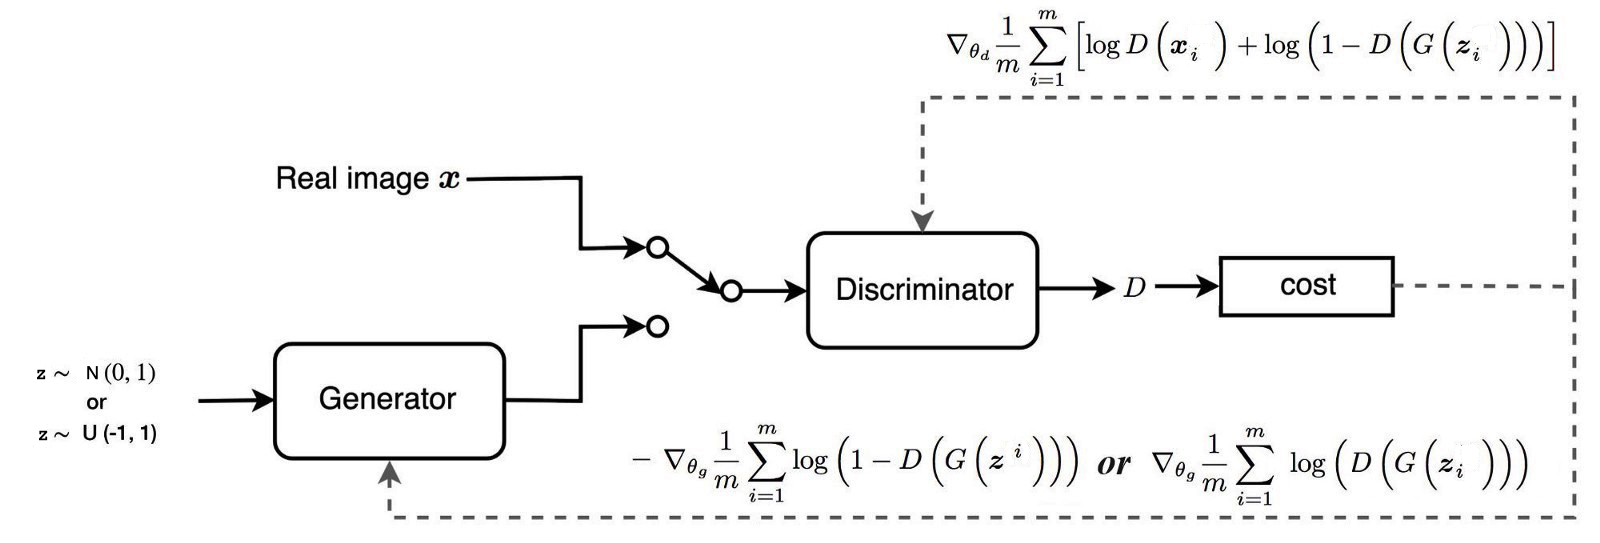
\includegraphics[]{figures/neural_networks/gan.jpeg}
	\end{adjustbox}
	\caption{Schematic diagram for Generative Adversarial Network\cite{ponti2017}.}\label{fig:gan}

\end{figure*}

\begin{figure}
    \centering

        \begin{tikzpicture}[start chain=going below, node distance=12pt,
            point/.append style={on chain, join=by {signal}},
            layer/.append style={on chain, join=by {signal}},
            branch/.append style={on chain, join=by {signal, -}},
            ]
            \def\branchy{20pt}

            \node[activation] {Layer 1};
            \node[branch] (input) {};
            \node[bn, xshift=\layerwidth/2+16pt, yshift=-\branchy] {Layer 2};
            \node[conv] {Layer 3};
            \node[layer, xshift=-\layerwidth/2-16pt, yshift=-\branchy] (add) {Layer 4};
            \node[point] {Output};
            \draw[signal] (input) -- (add);
        \end{tikzpicture}
    \caption{Skip connection connecting non-adjacent layers.}\label{fig:skipconnection}
\end{figure}
Another solution to the vanishing gradients problem is using \textit{skip connections}: outputs from non-adjacent layers are used as inputs for a layer (see figure~\ref{fig:skipconnections}).
%
This has the effect that substantive gradients can be propagated farther back into the network more easily (since they skip being attenuated by intermediate layers).

Overfitting is mititaged by using regularization; methods such as \(L_2\) regularization and \textit{dropout} have been shown to be effective against overfitting\cite{bengio2013}.
%
\(L_2\) regularization incorporates a squared weight term \(\frac{\lambda}{2}\sum_{i=1}^n w_i^2\) into eqn.~\eqref{eqn:loss}, which translates into a \textit{weight decay} term \(\lambda w_i^{t-1}\) in the Delta rule (eqn.~\eqref{eqn:sgd}):
\begin{equation}
    \Delta w_i^t = \alpha \cdot \sum_j (t_j-y(\mathbf{x}_j))\cdot \sigma'\cdot x_{ij} + \lambda w_i^{t-1}
    \label{eqn:weightdecaydelta}
\end{equation}
On the other hand dropout enforces regularization by selectively disabling neurons in the network (see figure~\ref{fig:dropout}); on each forward pass through the network a neuron is either passed input or not according to some probability \(p\) (usually \(p = 0.5\)).
%
The intuition being that not every neuron will have an opportunity to learn from every sample thereby limiting its, and the network's as a whole, ability to memorize patterns unique to the training samples (i.e., overfit).

Overfitting and vanishing gradients are not the only challenges encountered when training DNNs.
%
Hence there are many other best-practices techniques for training DNNs that are beyond the scope of this brief review; an accessible survey is Montavon \etal\cite{montavon2012neural}.
\subsubsection{Generative Adversarial Networks}\label{subsubsec:gan}
A Generative Adversarial Network\cite{goodfellow2014generative} is a training regimen for networks that perform \textit{generative tasks}.
%
A generative task is one which calls for generating samples from a probability distribution represented by the training data.
%
For example one might have many images of people and one might wish to generate new samples (see figure~\ref{fig:stylegan}) from the probability distribution of such images (i.e., new images of people).
\begin{figure}
    \centering
    \begin{adjustbox}{width=\linewidth}
        \centering
        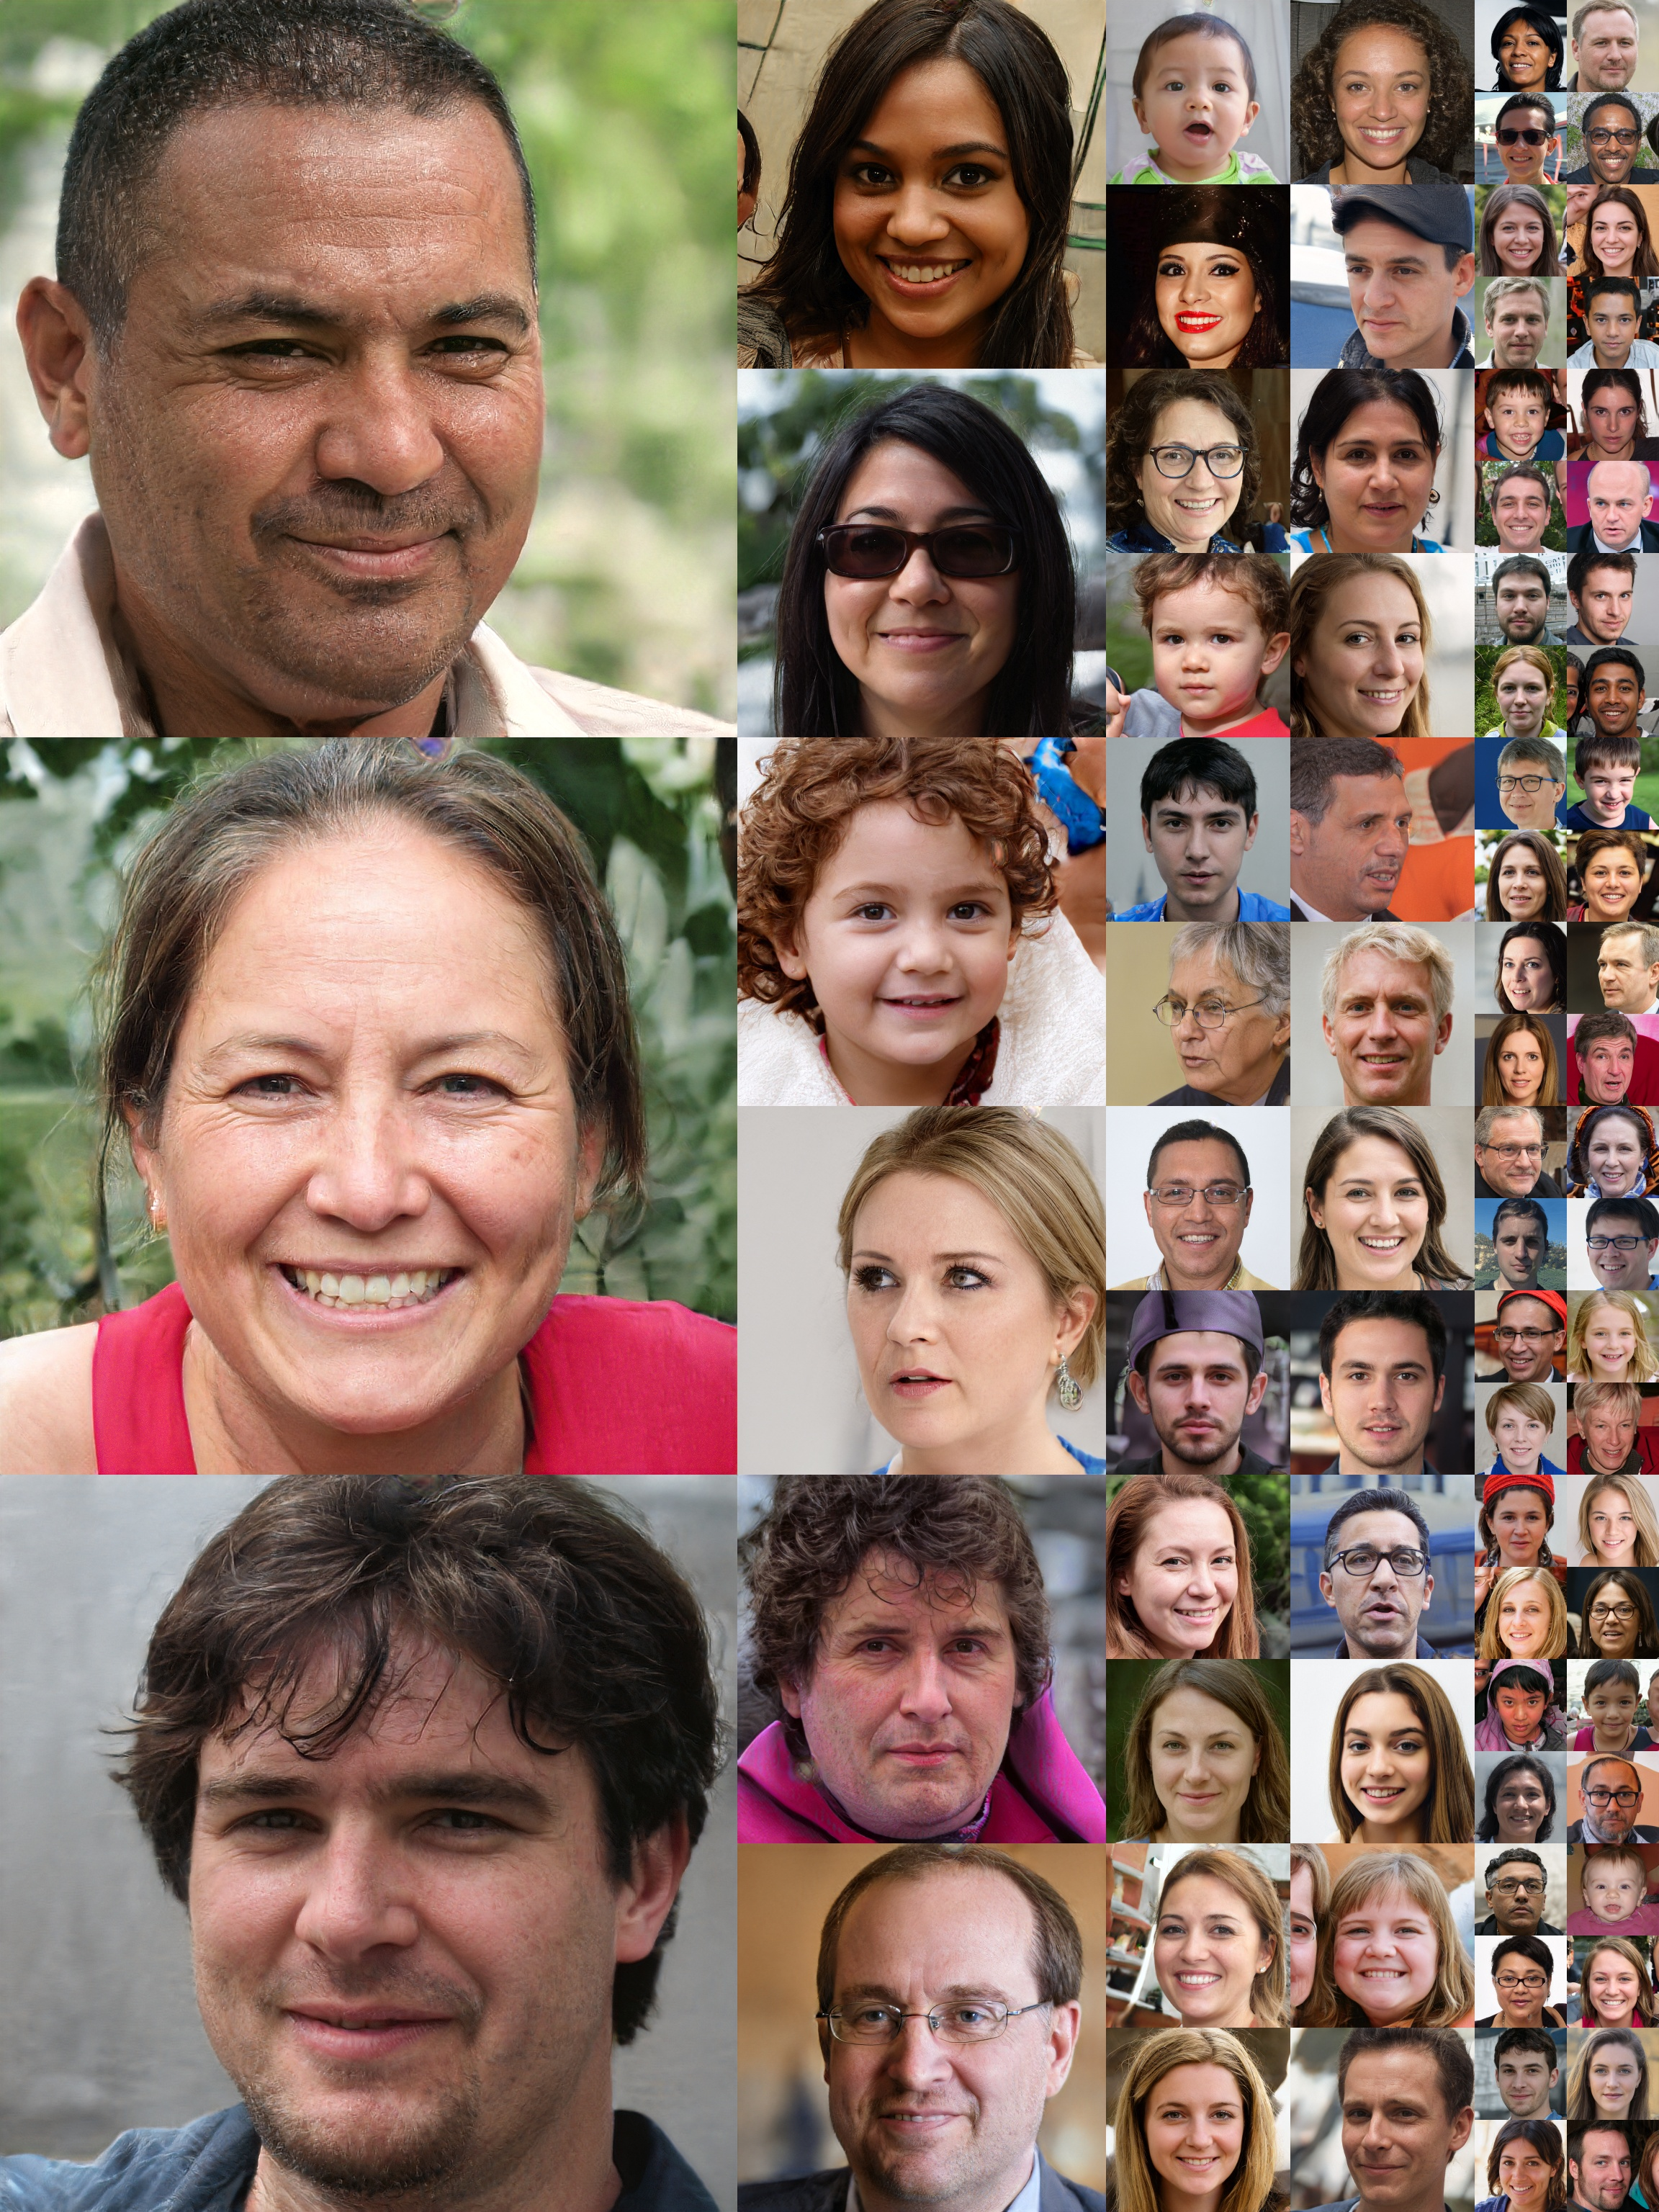
\includegraphics[]{figures/neural_networks/stylegan.jpg}
    \end{adjustbox}
    \caption{Uncurated set of images \textbf{generated} (i.e., none of the people depicted are real) using StyleGAN with the FFHQ dataset\cite{karras2018stylebased}.}\label{fig:stylegan}
\end{figure}
%
In general this is a highly non-trivial problem due to the dimensionality of the sample space.

GANs solve this problem by pitting a \textit{generator} \(G\), that learns to transform samples from a readily available high-dimensional surrogate distribution (Normal or Uniform), against a \textit{discriminator} \(D\).
The generator takes as input samples \(\bm{z}\) from the surrogate distribution \(p_{\bm{z}}\) and outputs putative samples \(G(\bm{z})\) from the desired distribution.
%
The discriminator alternates between considering true samples \(\bm{x}\) from the desired distribution \(p_r\) and considering counterfeit samples \(G(\bm{z})\) produced by the generator; it therefore assesses the quality of \(G\)'s output with respect to its own understanding of the desired distribution.
%
To that end Goodfellow \etal\cite{goodfellow2014generative} propose a training framework that involves playing a \textit{mini-max game}\anote{minimax}:
\begin{equation}
    \min_G \max_D L(D, G)
\end{equation}
where
\begin{multline}
    L(D, G) \coloneqq \mathbb{E}_{\bm{x} \sim p_{r}} [\log D(\bm{x})] + \\ \mathbb{E}_{\bm{z} \sim p_{\bm{z}} } [\log(1 - D(G(\bm{z})))]
    \label{eqn:ganloss}
\end{multline}
Since the discriminator seeks to maximize \(L(D, G)\), the term \(\mathbb{E}_{\bm{x} \sim p_{r}} [\log D(\bm{x})]\) ensures that it's able to correctly identify (i.e., score high) true samples.
%
Simultaneously the term \(\mathbb{E}_{\bm{z} \sim p_{\bm{z}} } [\log(1 - D(G(\bm{z})))] \) ensures that it's able to correctly identify (i.e., score low) counterfeit samples produced by \(G\).
%
On the other hand the inverse holds for \(G\) with respect to \(\mathbb{E}_{\bm{z} \sim p_{\bm{z}} } [\log(1 - D(G(\bm{z})))]\) (the first term in eqn.~\eqref{eqn:ganloss}) does not play a role when optimizing \(G\)) and so \(G\) improves in its ability to fool the discriminator (i.e., produce plausible samples from the desired distribution).
%
Goodfellow \etal go on to prove that for the generator this loss criterion is equivalent to minimizing the Jensen–Shannon divergence\anote{kldiv} between the distribution that it represents and the desired, true, distribution of the data.
\subsection{Deep Neural Networks for SISR}
Deep neural network architectures for single-image super-resolution abide a four tiered hierarchy (according to complexity) which roughly parallels the chronological order of the innovations that have contributed to the current state of the art:
\begin{framed}
    \begin{itemize}
        \item \textbf{Pre-defined up-sampling}: networks that expect the image to already have been up-sampled (e.g., using bicubic interpolation). These networks chiefly restore high-frequency features that are omitted by the classical up-sampling technique.
        \item \textbf{Single up-sampling}: networks that perform the up-sampling themselves (in addition to performing restoration).
        \item \textbf{Progressive up-sampling}: networks that up-sample in phases, performing restoration at every phase.
        \item \textbf{Iterative up-sampling}: networks that up-sample and then assess the goodness of the result by down-sampling to original low-resolution (see section~\ref{subsubsec:iterback} for the classical analogue).
    \end{itemize}
\end{framed}
\subsubsection{SRCNN and Very Deep SR}\label{subsubsec:vdsr}
The first successful foray of Deep Learning was the 2-layer Super-Resolution CNN (SRCNN) model\cite{Dong_2016}.
%
SRCNN is a CNN composed of two convolution layers, with the first layer consisting of 64 filters (per color channel), the second layer consisting of 32 filters, and both layers employing \(\operatorname{ReLU}\) activations.
%
\begin{figure}
    \centering
    \newcommand*{\subfigwidth}{0.49\textwidth}
    \begin{subfigure}[b]{\subfigwidth}
        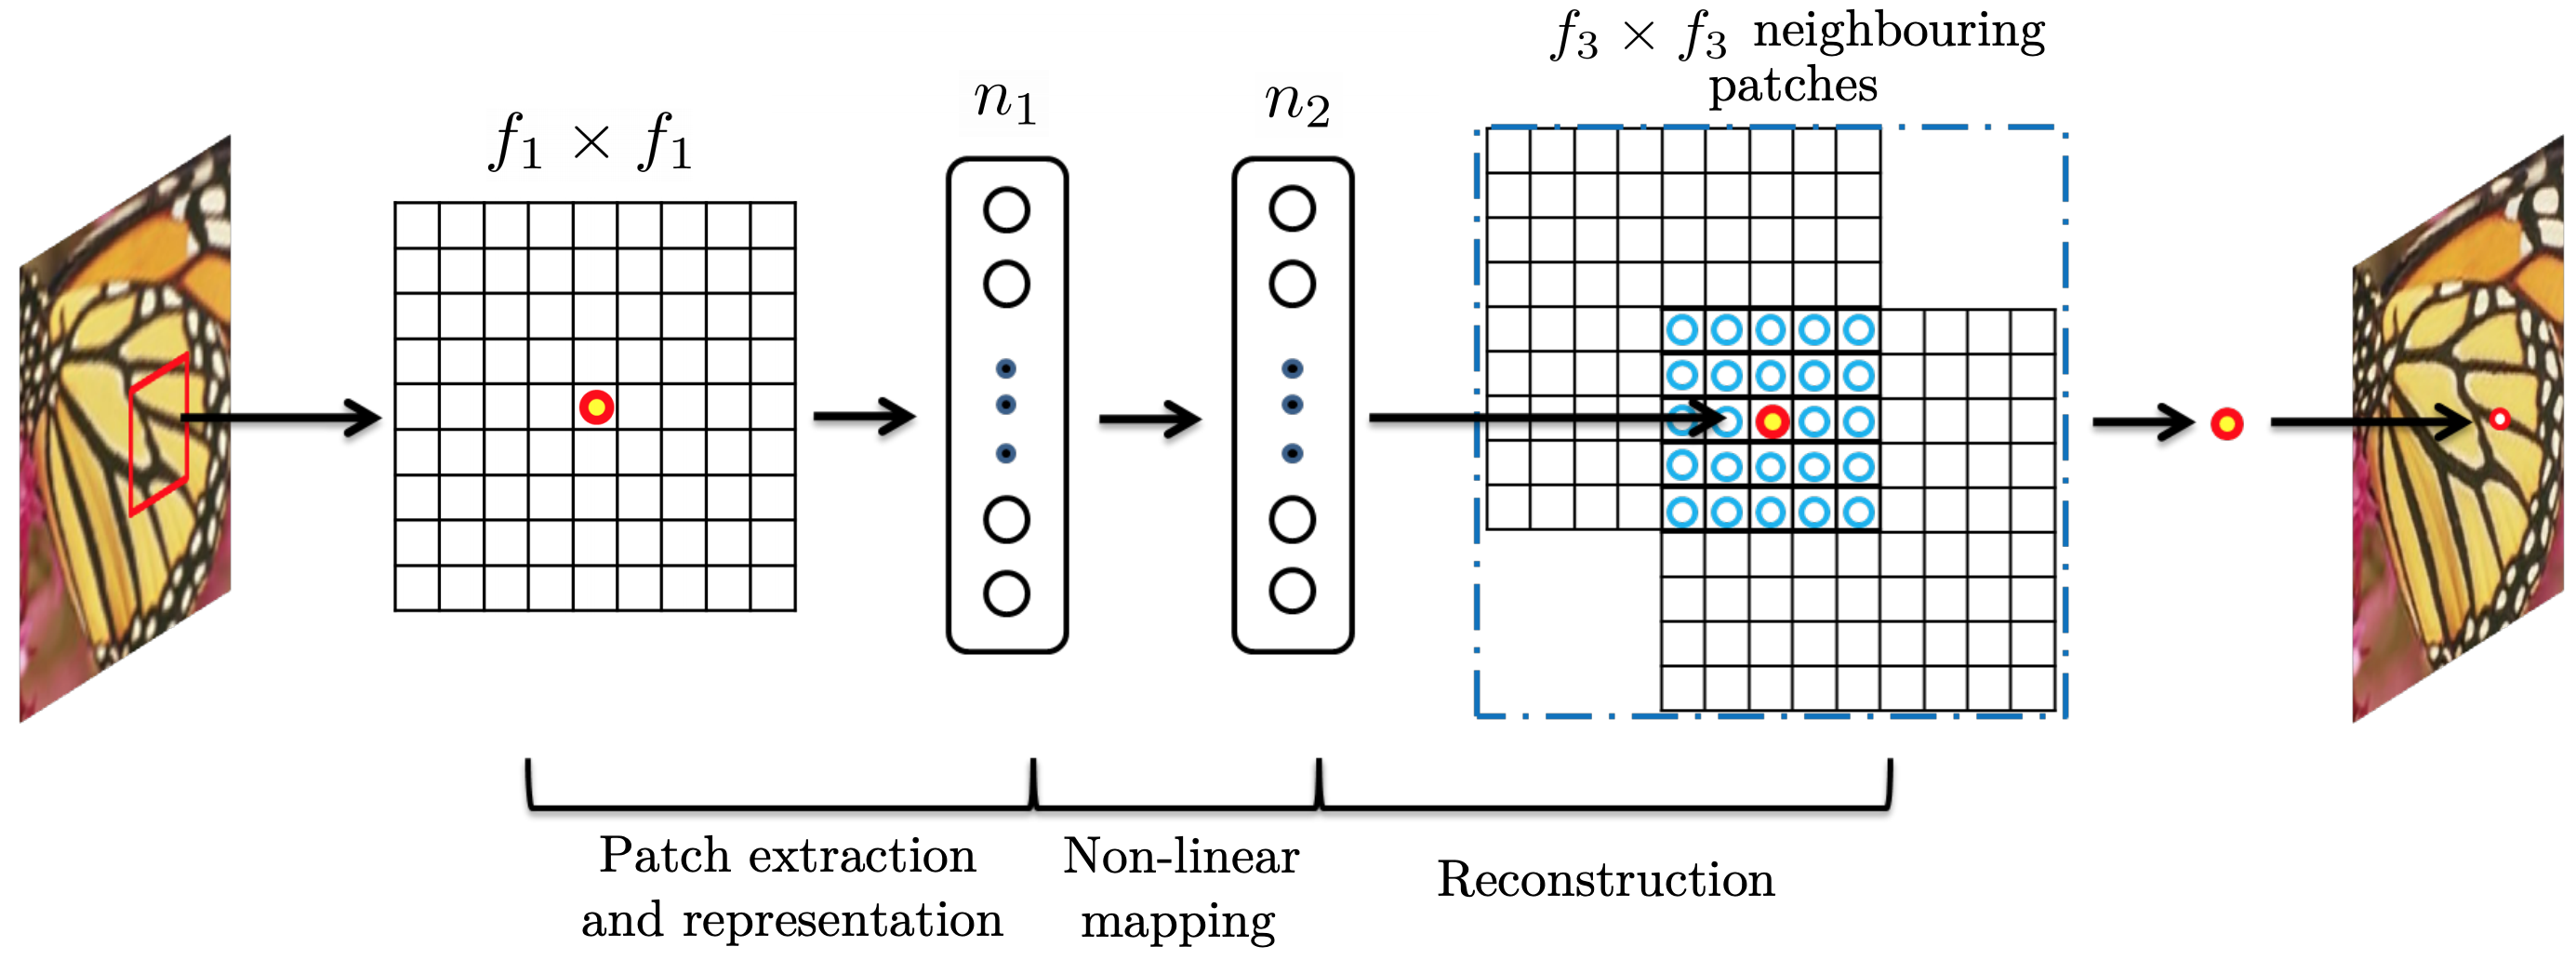
\includegraphics[width=\linewidth,keepaspectratio]{figures/neural_networks/sparse_coding.png}
        \caption{Sparse coding SR pipeline (see section~\ref{subsubsec:sparsecoding}).}\label{subfig:srcnnsparse}
    \end{subfigure}
    \vskip\baselineskip
    \begin{subfigure}[b]{\subfigwidth}
        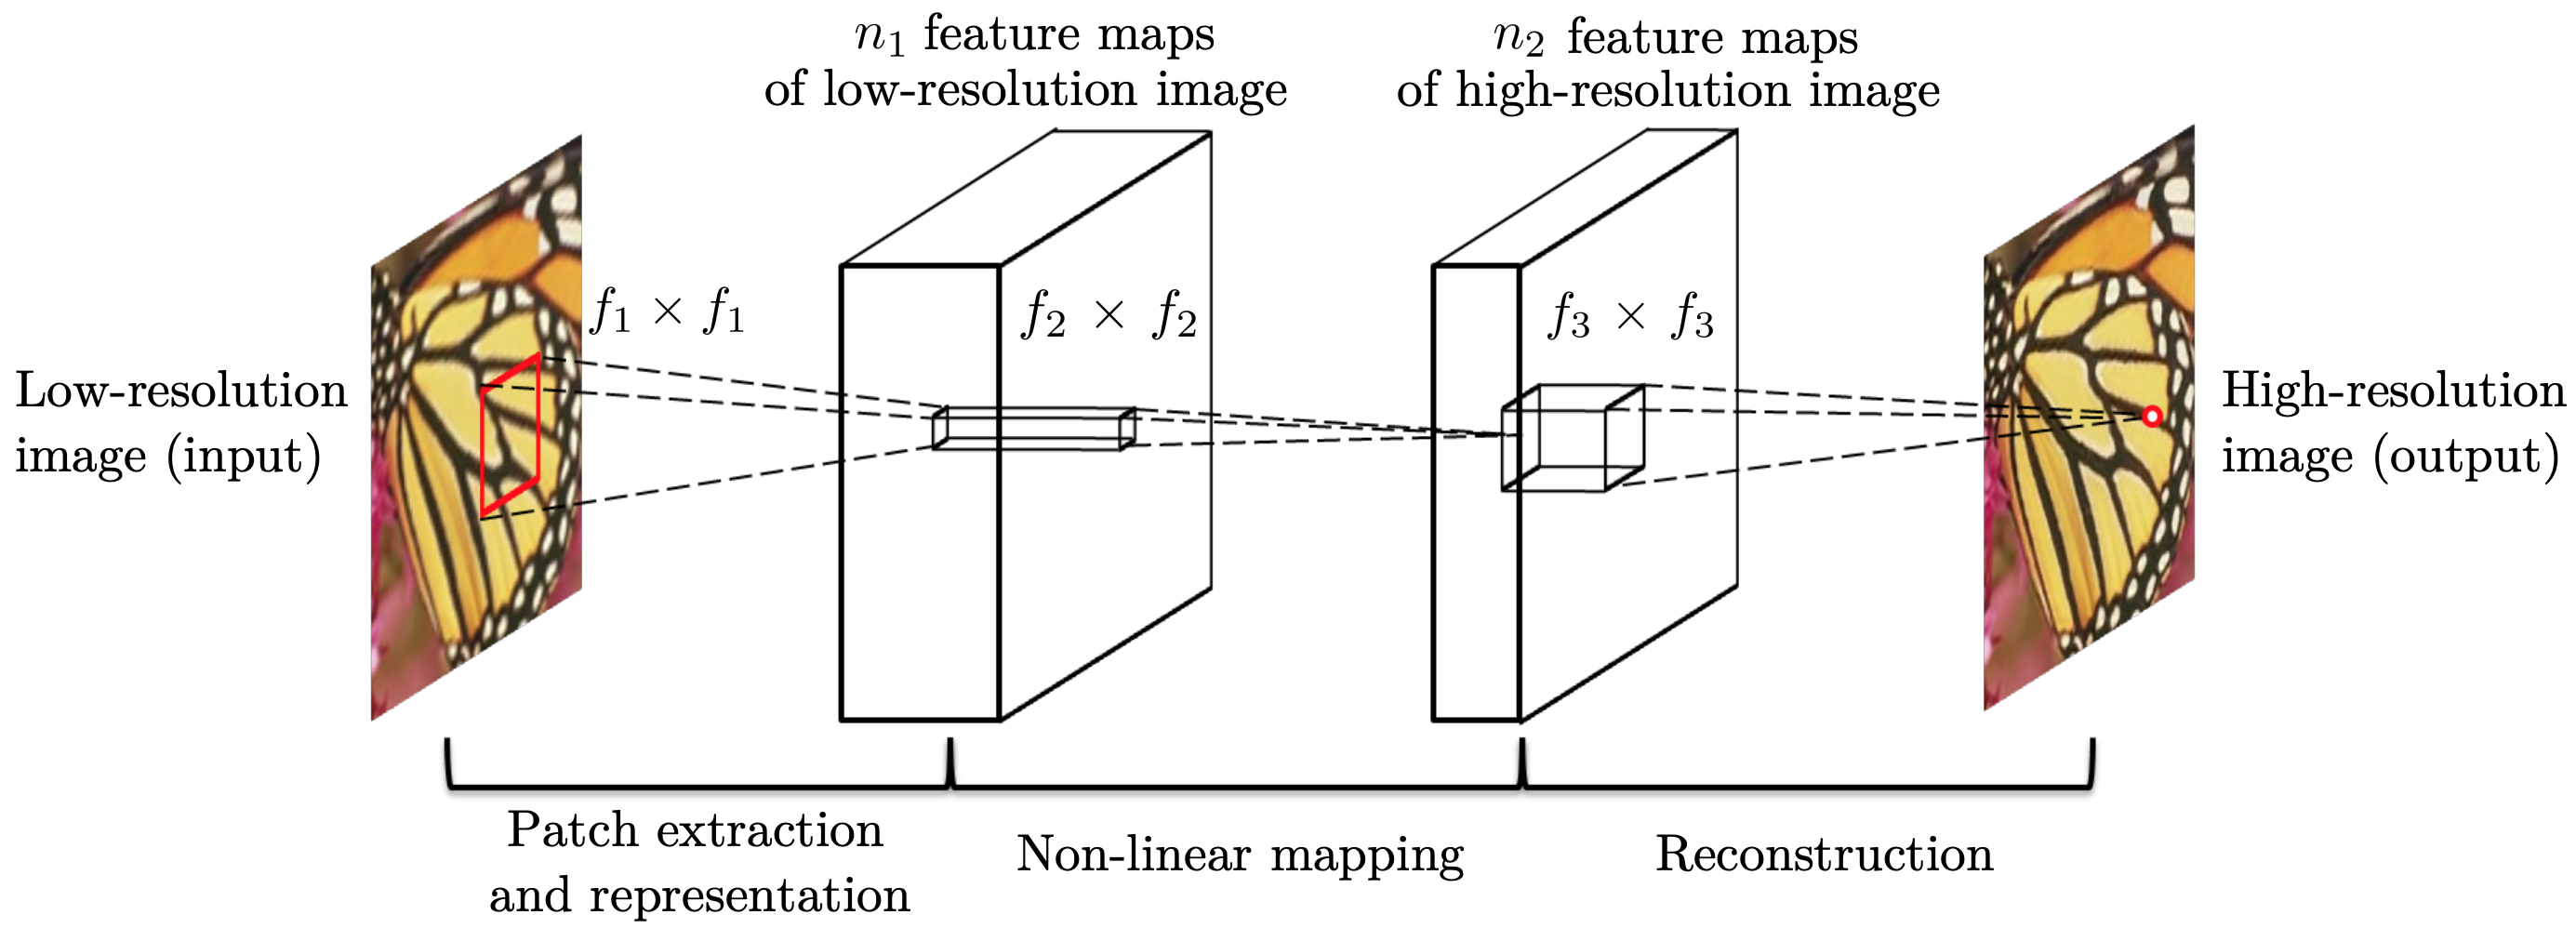
\includegraphics[width=\linewidth,keepaspectratio]{figures/neural_networks/srcnn.png}
        \caption{SRCNN pipeline.}\label{subfig:srcnn}
    \end{subfigure}
    \caption{Sparse coding SR and SRCNN comparison\cite{Dong_2016}. Note both pipelines operate on bicubic up-sampled images.}\label{fig:srcnn}
\end{figure}
Dong \etal argue that their CNN architecture is equivalent to sparse coding SR (see figure~\ref{fig:srcnn}).
%
This is a common theme in the literature --- ANN architectures learning transformations equivalent to classical techniques --- owing to the universal approximation theorem.

Clearly, at least by modern standards, 2 layers isn't very deep; Dong \etal do experiment with an additional convolution layer but report difficulties maintaining reasonable convergence rates due to vanishing gradients.
%
Kim \etal\cite{Kim_2016} improve on SRCNN with Very Deep SRCNN (VDSR) by increasing the convolution layer count to a sum total of 20.
%
In order to overcome the training challenges faced by Dong \etal they use skip connections (see section~\ref{subsubsec:dnns}).
%
They also use learning rate \textit{annealing}\anote{annealing} and implement gradient clipping to prevent \textit{exploding gradients}\anote{gradclip}.
%
They further argue that an SR network need only learn \textit{residuals} \(\bm{r} \coloneqq \bm{t} - \bm{x}\).
%
In this context, residuals have the significance of being the high-frequency components of an image, since the bicubic up-sampled input \(\bm{x}\) can be interpreted as a low-pass filtered version of the high-resolution image.
%
Hence, their loss function measures the error between the HR image target and the output of the network \(\bm{y}\) plus the input:
\begin{equation}
    L \coloneqq \abs{\bm{t} - (\bm{x} + \bm{y})}^2
\end{equation}

\subsubsection{Super-Resolution GAN}\label{subsubsec:srgan}
Single up-sampling networks forgo bicubic pre-processing and learn the up-sampling transformation as a component of the network.
%
The most interesting network in this class of networks is the Super-resolution Residual Network (SRResNet) along with its GAN trained counterpart SRGAN\cite{Ledig_2017}.
%
SRResNet takes as input LR images and similar to VDSR passes them through 16 individual ResBlocks (see figure~\ref{fig:resblock}) for feature extraction.
%
Where SRResNet differs from VDSR is the in-network up-sampling that it performs using \textit{sub-pixel convolutions}.
%
Sub-pixel convolutions are a way to learn up-sampling as a component of the ANN.
\begin{figure}
    \centering
    \newcommand*{\subfigwidth}{.49\textwidth}
    \begin{subfigure}[b]{\subfigwidth}
        \centering
        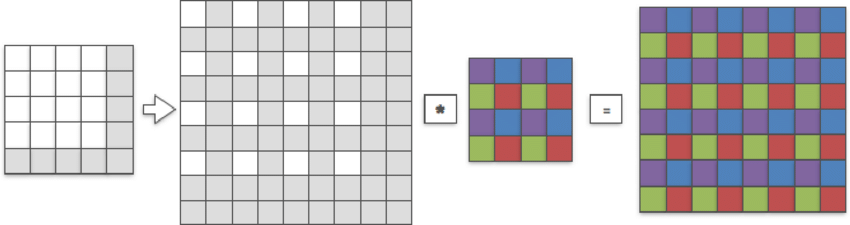
\includegraphics[width=\textwidth]{figures/neural_networks/subpixelconv1.png}
        \caption{Sub-pixel convolution as dilation then filtering.}\label{subfig:subpixdilate}
    \end{subfigure}
    \vskip\baselineskip
    \begin{subfigure}[b]{\subfigwidth}
        \centering
        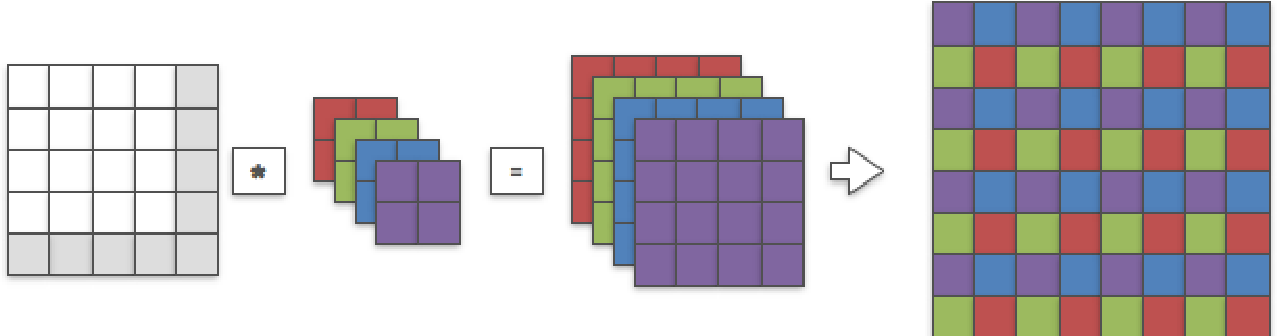
\includegraphics[width=\textwidth]{figures/neural_networks/subpixelconv2.png}
        \caption{Sub-pixel convolution as filtering then pixel-shuffling.}\label{subfig:pixelshuffle}
    \end{subfigure}
    \caption{Sub-pixel convolution.}\label{fig:subpixelconv}
\end{figure}
%
The up-sample in two phases: first \(r^2\) filters are convolved with the input, where \(r\) is up-sampling factor (e.g., 4 filters for 2x up-sampling), then a \textit{pixel shuffle} operation places the entries of the feature maps in an \(r\)-times higher resolution grid (see figure~\ref{subfig:pixelshuffle}).
%
This operation is called a sub-pixel convolution because it can be interpreted as first dilating the LR image and then convolving with a filter to get a feature map with sub-pixel (relative to the original LR image) responses (see figure~\ref{subfig:subpixdilate}).

Ledig \etal pre-train SRResNet using mean-squared-error (MSE) loss and then further train using the GAN framework (see section~\ref{subsubsec:gan}).
%
\begin{figure}
    \centering
    \begin{adjustbox}{width=\linewidth}
        \centering
        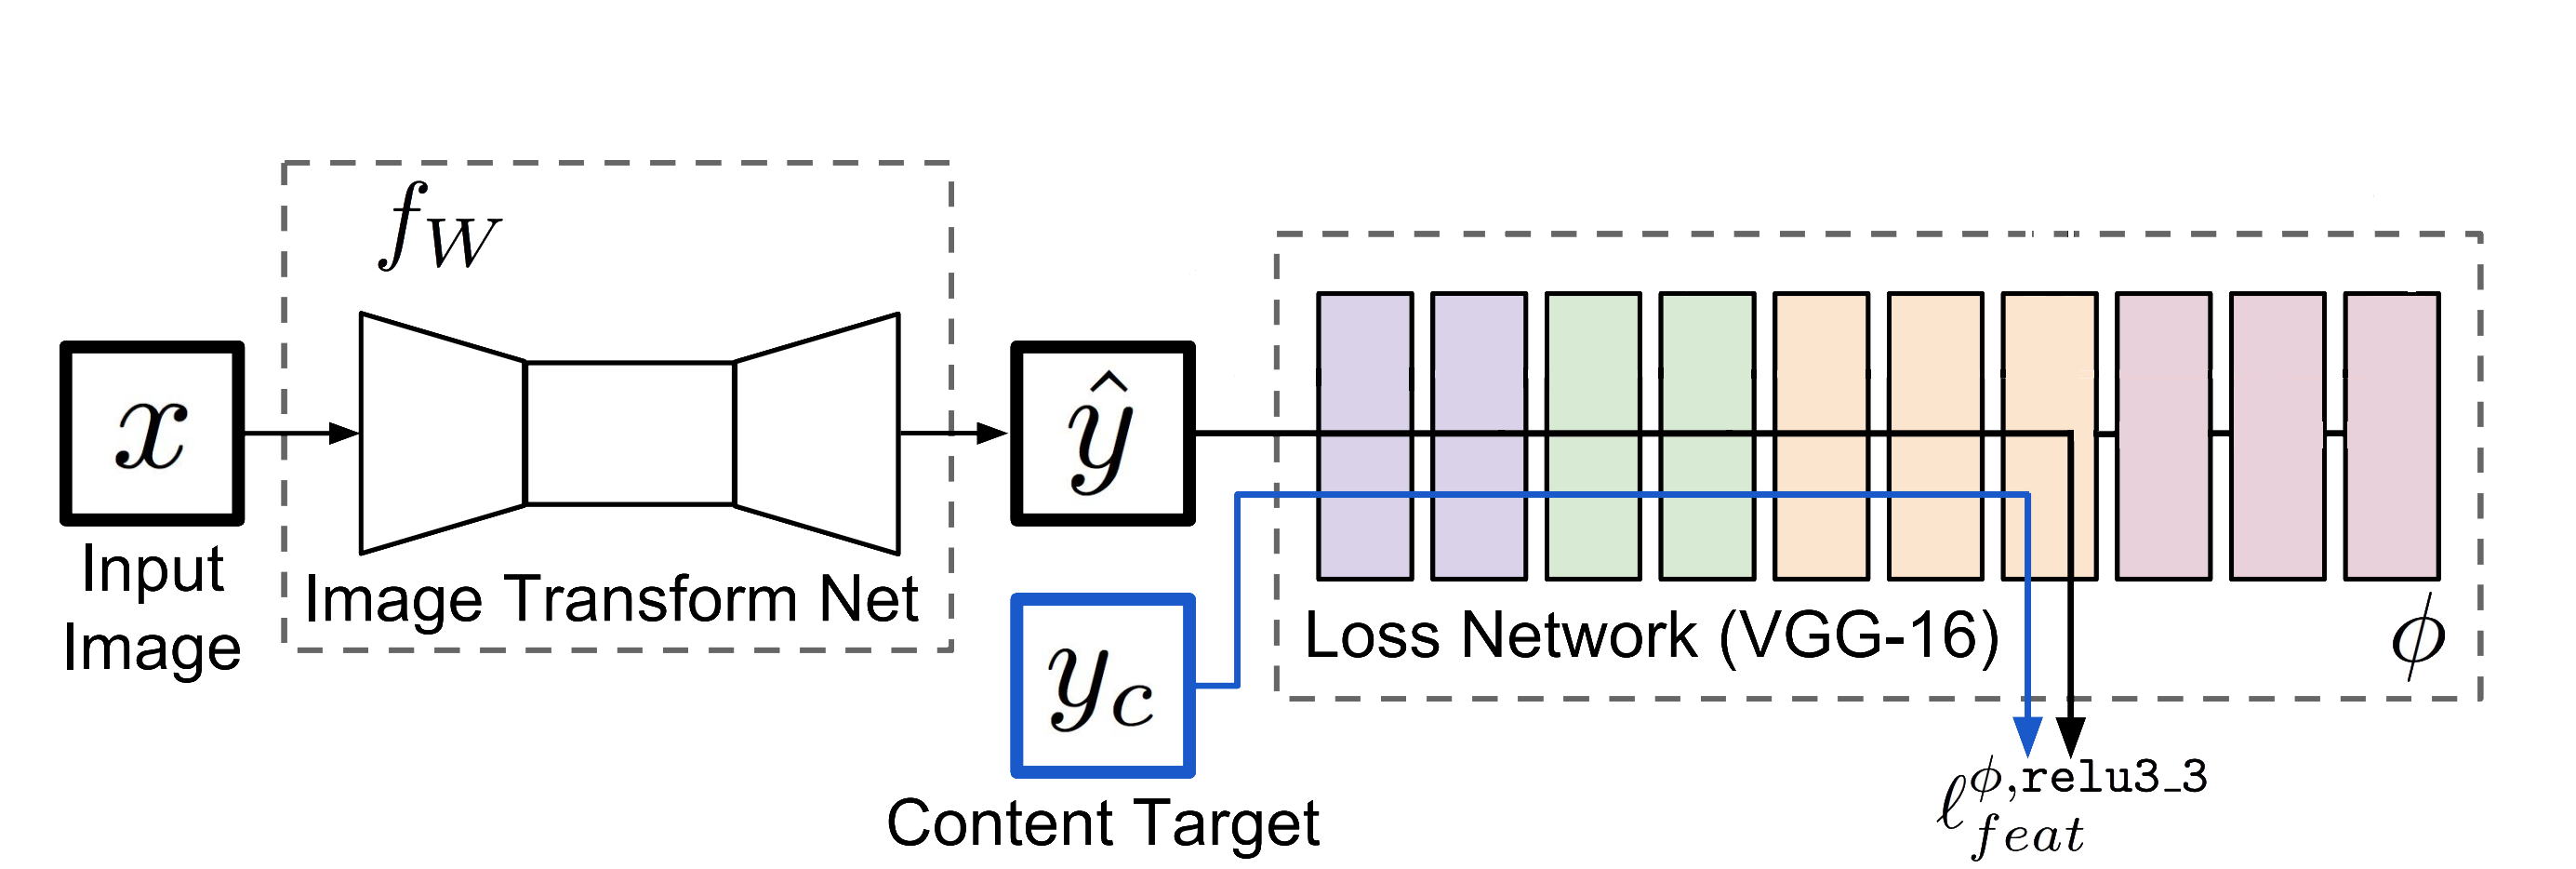
\includegraphics[]{figures/neural_networks/perceptual_loss.png}
    \end{adjustbox}
    \caption{Perceptual loss\cite{johnson2016perceptual}.}\label{fig:perceptualloss}
\end{figure}
In addition to using the conventional GAN loss they add a term they call \textit{perceptual loss}:
\begin{equation}
    \ell_{feat}^{\phi, j} \left( \hat{\bm{y}}, \bm{y}_c\right) \coloneqq \frac{1}{H_j W_j} \abs{\phi_j\left({\hat{\bm{y}}}\right) - \phi_j \left(\bm{y}_c\right)}^2
\end{equation}
where \(\phi_j\) is the \(j\)th layer activation of the VGG network\cite{simonyan2014very} pretrained on a large data set, \(\hat{\bm{y}}\) is the output of SRResNet, and \(\bm{y}_c\) is the target HR image (see figure~\ref{fig:perceptualloss}), and \(H_j, W_j\) are the dimensions of the \(j\)th layer activation of VGG.
%
They argue that this loss is closer to perceptual similarity than MSE loss and therefore encourages reconstruction of high frequency content that MSE loss alone suppresses.
\subsubsection{Laplacian Pyramid Super-Resolution Network}\label{subsubsec:lapsrn}
\begin{figure}
    \centering
    \begin{adjustbox}{width=\linewidth}
        \centering
        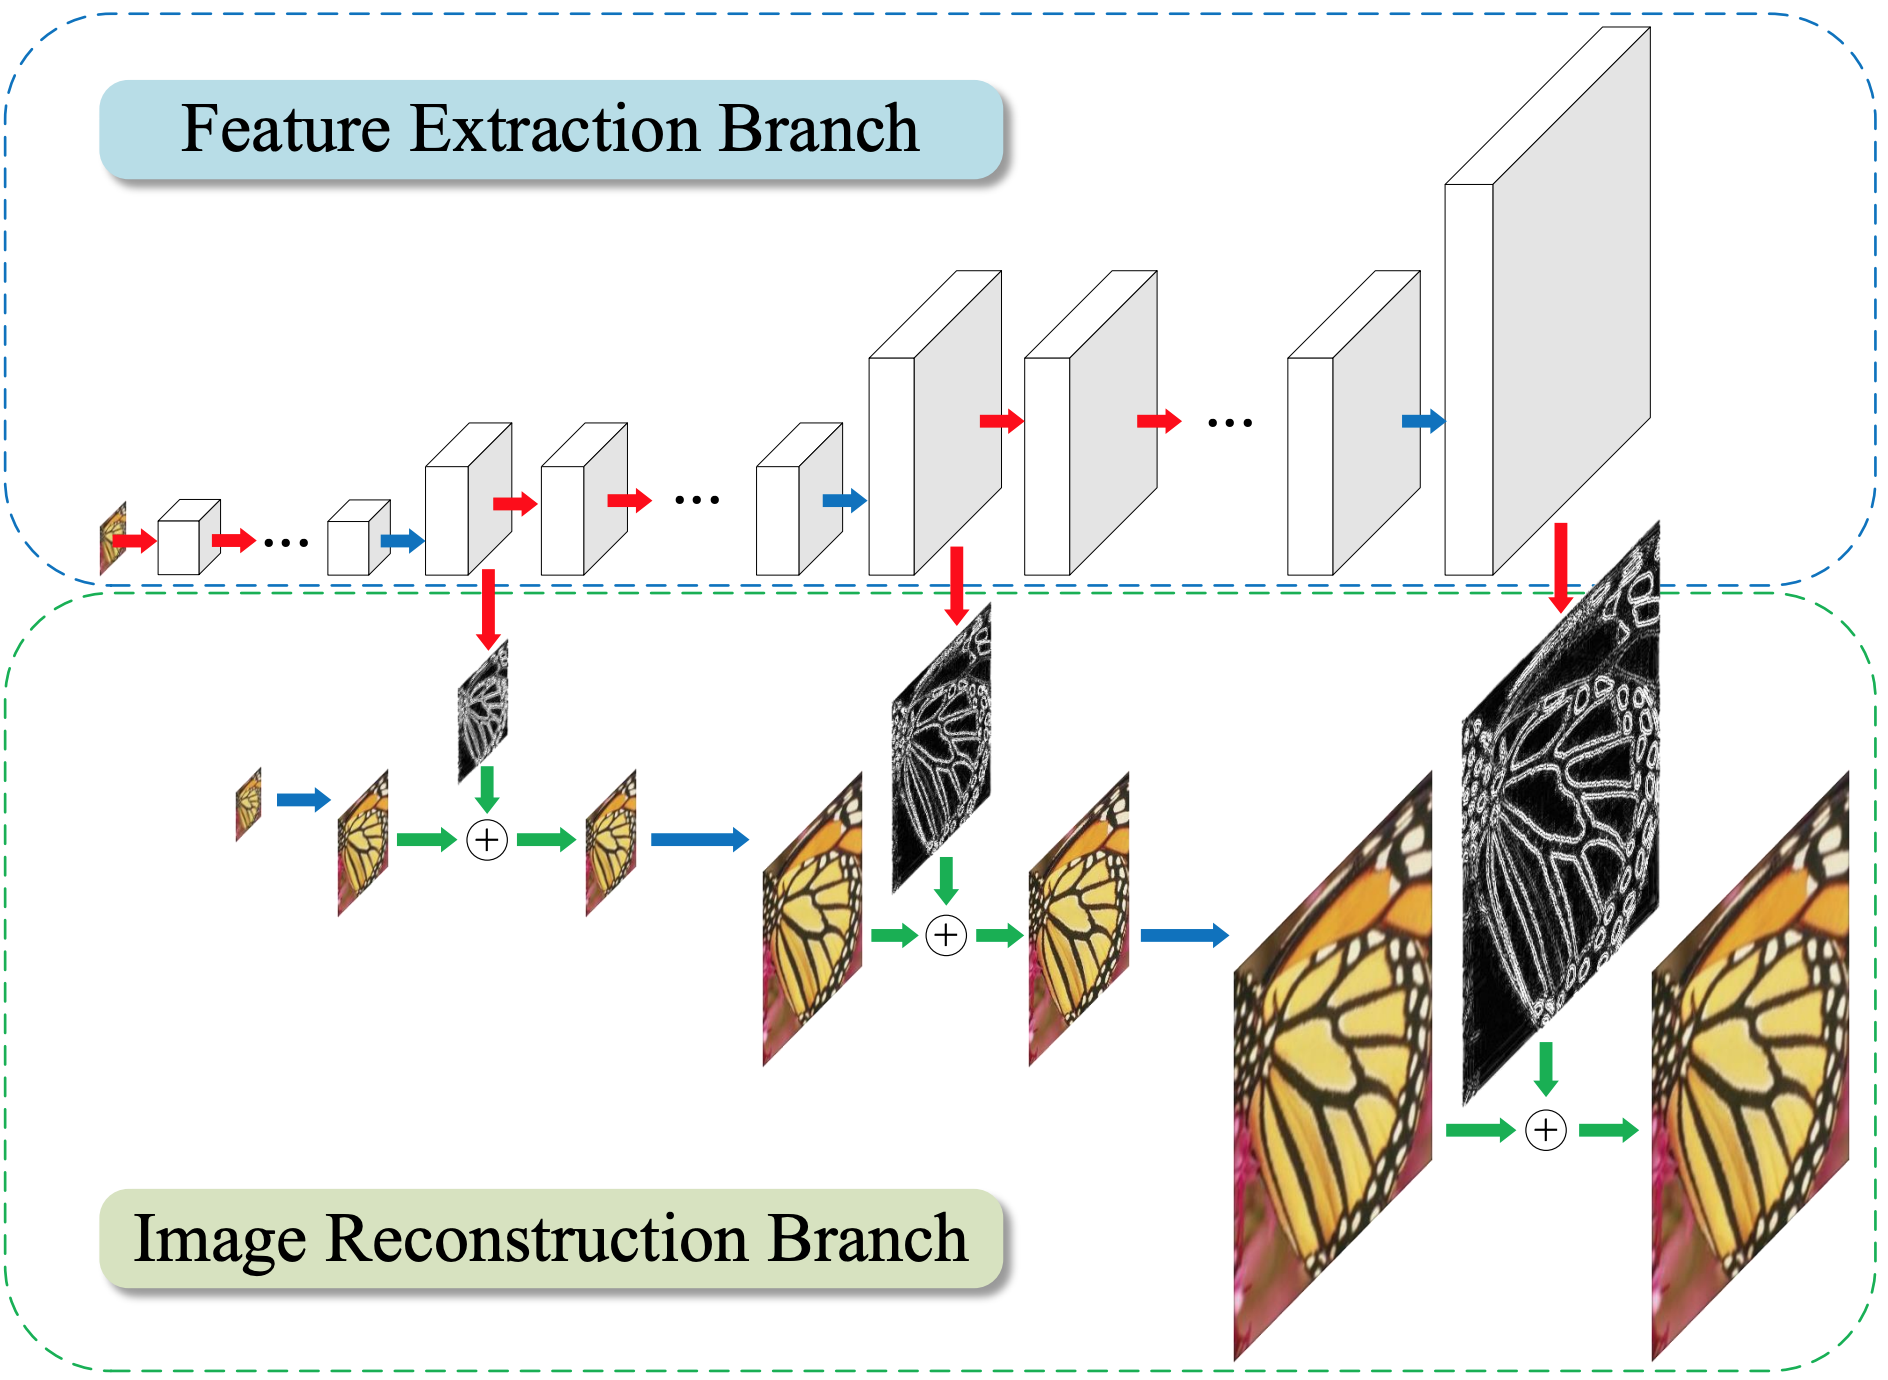
\includegraphics{figures/neural_networks/lapsrn.png}
    \end{adjustbox}
    \caption{LapSRN architecture\cite{Lai_2017}.}\label{fig:lapsrn}
\end{figure}
Lai \etal\cite{Lai_2017} propose a network that up-samples by predicting sub-band (see section~\ref{subsubsec:subband}) residuals at progressively finer and finer scales (i.e., higher and higher resolution).
%
Their network consists of \(\log_2(r)\), where \(r\) is the scaling factor, tiers of CNNs along two branches: a feature extraction branch and an image reconstruction branch (see figure~\ref{fig:lapsrn}).
%
For a given tier the feature extraction branch extracts the gradients that comprise the residual and performs a 2x up-sampling (using transposed convolution). 
%
The output of the feature extraction branch, at a given tier, is then passed on to the next feature extraction tier and simultaneously to the corresponding image reconstruction tier.
%
The image reconstruction branch, at a given tier, up-samples the input image (also using transposed convolution) and element-wise sums it to the residual produced by the feature extraction branch (at the corresponding tier).
%
This structure emulates a Laplacian pyramid (see figure~\ref{fig:bertrand}) along both branches and as a result is called the Laplacian Pyramid Super-Resolution Network (LapSRN).

They also identify \(L_2\) loss as a source of perceptual fidelity flaws and substitute Charbonnier loss\cite{charbonnier1994two} \(\rho(\bm{x})\) to train their network:
\begin{equation}
    \rho(\bm{x}) \coloneqq \sqrt{\frac{\bm{x}\cdot \bm{x}}{\epsilon^2}+ 1}
\end{equation}
where \(\epsilon\) is a scale parameter that they empirically set to \(10^{-3}\). 
%
Lie \etal train their network using \textit{deep supervision}; the loss function they optimize compares the result at every tier of the network against the target HR image (the HR image is down-sampled to produce targets at multiple scales):
\begin{equation}
    L(\bm{t}, \bm{y}) \coloneqq \sum_{i=1}^{\log_2(r)} \rho(\bm{t}_i - \bm{y}_i)
\end{equation}
where \(\bm{t}_i \coloneqq (t_{\log_2{(r)}}, \dots, t_1)\) is the target HR image down-sampled and \(\bm{y} \coloneqq (y_1, \dots, y_{\log_2(r)})\) are the outputs of LapSRN at each of the tiers.
\subsubsection{Deep Back-Projection Networks}\label{subsubsec:dbpn}
\begin{figure}
    \centering
    \newcommand*{\subfigwidth}{0.49\textwidth}
    \begin{subfigure}[b]{\subfigwidth}
        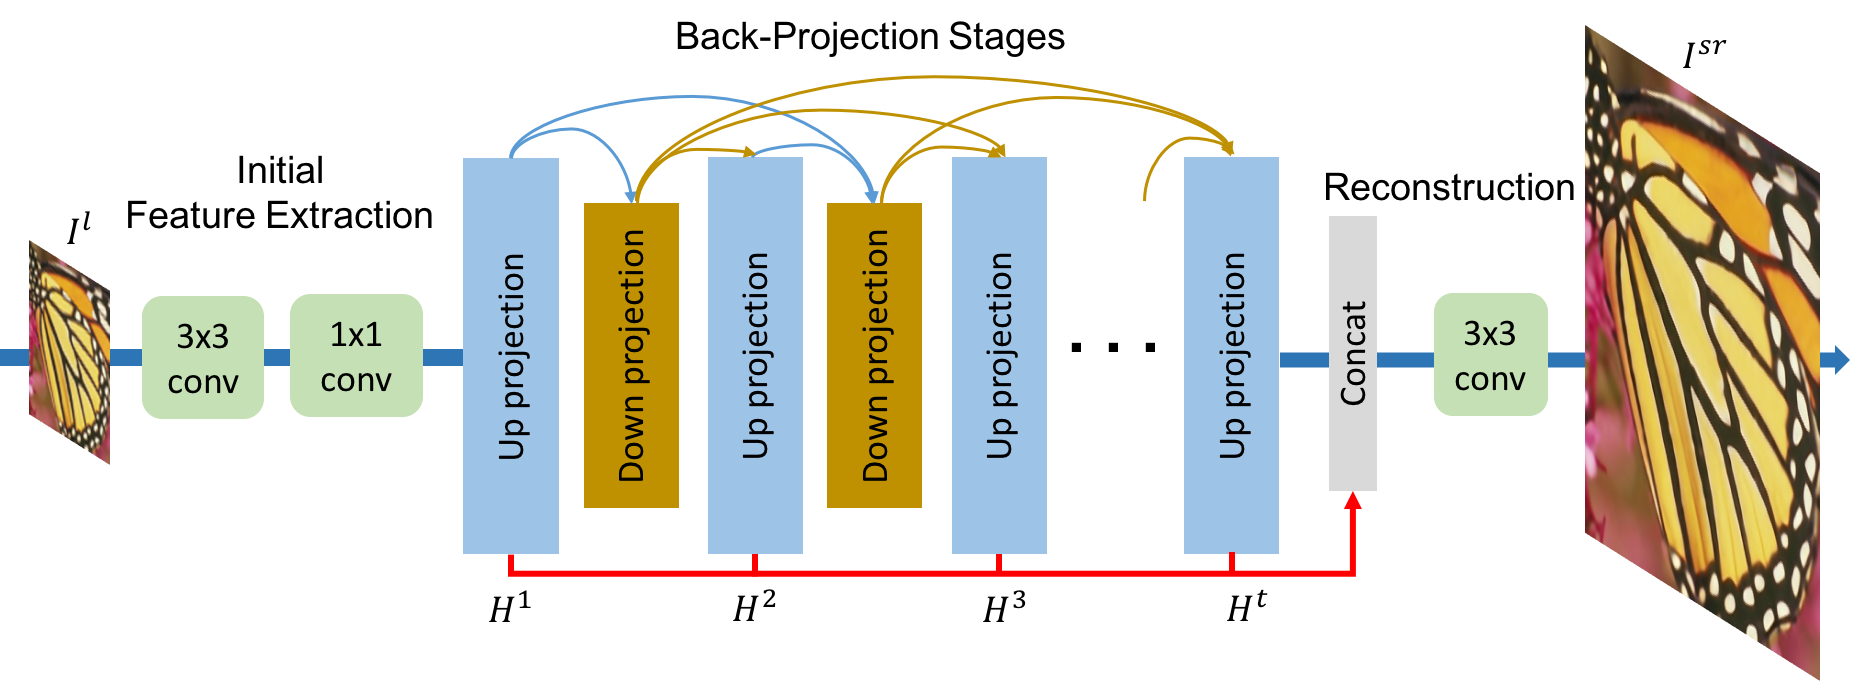
\includegraphics[width=\linewidth,keepaspectratio]{figures/neural_networks/DBPN.png}
        \caption{End-to-end DBPN network.}\label{subfig:dbpn}
    \end{subfigure}
    \vskip\baselineskip
    \begin{subfigure}[b]{\subfigwidth}
        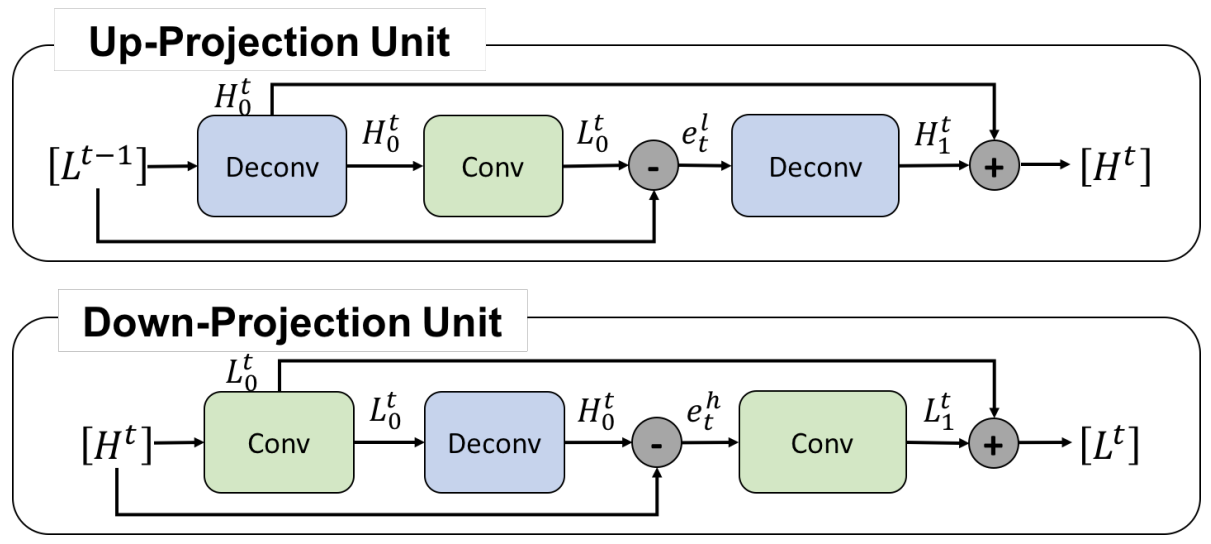
\includegraphics[width=\linewidth,keepaspectratio]{figures/neural_networks/up_down_up.png}
        \caption{DBPN Up, Down projection unit components implementing error correction.}\label{subfig:updowndbpn}
    \end{subfigure}
    \caption{Deep Back-Projection Networks \cite{haris2018deep}.}\label{fig:srcnn}
\end{figure}
Inspired by recent theories on the function of the human visual cortex\cite{kravitz2013ventral} Harris \etal\cite{haris2018deep} propose a deep neural network for SR that incorporates error-correcting feedback mechanisms.
%
They build on the work of Irani \etal (see section~\ref{subsubsec:iterback}) and implement deep iterative back projections (DBPN) (see figure~\ref{subfig:dbpn}).
%
These iterative back-projections are in effect repeated up-down-up sampling units, implemented using skip connections and deconvolutions, that minimize reconstruction error (see figure~\ref{subfig:updowndbpn}).
%
In classical iterative back projection a sequence of LR images is used to estimate an HR image.
%
Harris \etal use only a single input LR image and produce multiple candidate HR images uses multiple learned up-sampling operators (deconvolutions).
%
Their Up-Projection units take the error \(e_t^l\) between a proposed up-sampling \(H_0^t\) and the back-projection \(L_0^t\) and feeds it back into the proposed up-sampling, i.e., the error-correcting feedback is the difference between the back-projection and LR input.
%
Their Down-Projection units perform the same function but from HR to LR.
%
Using these units they achieve state of the art up-sampling all the way up to 8x\cite{timofte2018ntire}.
\subsection{Deep Neural Networks for MISR}
MISR algorithms process a batch of LR images to generate a single HR image by aggregating non-redundant information across the LR images.
%
In order to effectively perform this task they must compensate for motion between the LR images by registering them to a common pixel grid (see section~\ref{sec:registration}).
%
In the context of neural networks this is framed as learning the time dependency from the training data (LR-HR image pair sequences) and then inferring such a time dependency on new samples.
%
\subsubsection{Bi-directional Recurrent CNN}
    \begin{figure*}[!htbp]
        \centering
        	\begin{adjustbox}{width=\textwidth}

        \begin{tikzpicture}
            \def\nodedist{64pt}

            \node[block, fill=snowymint, rounded corners, minimum width=40pt, minimum height=24pt] (at) at (0,0) {A};
            \node[inputnode, below=26pt of at] (xt) {$x$};
            \node[outputnode, above=26pt of at] (ht) {$h$};
            \draw[signal] (xt) -- (at);
            \draw[signal] (at) -- (ht);
            \coordinate (0t) at ($(ht)!0.6!(at)$);
            \draw[signal, -, shorten >=\intergape] (at) -- node[below] {$t$} +(40pt,0pt) |- (0t);
            \draw[signal, latex-, shorten >=\intergape] (at) -- +(-40pt,0pt) |- (0t);

            \newcommand{\timestep}[2]{
                \node[block, fill=snowymint, rounded corners, minimum width=40pt, minimum height=24pt] (a#2) at #1 {A};
                \node[inputnode, below=26pt of a#2] (x#2) {$x_#2$};
                \node[outputnode, above=26pt of a#2] (h#2) {$h_#2$};
                \draw[signal] (x#2) -- (a#2);
                \draw[signal] (a#2) -- (h#2);
            }

            % \timestep{(0, 0)}{t};

            \node[] (e) at ($(at) +(\nodedist,0)$) {\LARGE=};

            \timestep{($(e) +(0.7*\nodedist,0)$)}{0};
            \timestep{($(a0) +(\nodedist,0)$)}{1};
            \draw[signal] (a0) -- (a1);
            \timestep{($(a1) +(\nodedist,0)$)}{2};
            \draw[signal] (a1) -- (a2);
            \timestep{($(a2) +(\nodedist,0)$)}{3};
            \draw[signal] (a2) -- (a3);

            \node[] at ($(a3) +(0.6*\nodedist,0)$) (ddd) {$\dots$};
            \timestep{($(ddd) +(0.7*\nodedist,0)$)}{t};
            \draw[signal, -] (a3) -- (ddd);
            \draw[signal] (ddd) -- (at);
        \end{tikzpicture}
    \end{adjustbox}
    \caption{\(t\)-step RNN unrolled.}\label{fig:unrolledrnn}
    \end{figure*}
    % \begin{subfigure}[b]{.49\textwidth}
    %     \centering
    %     \begin{tikzpicture}[thick, node distance=30pt and 30pt, on grid]
    %         \node[cell, minimum width=200pt, minimum height=110pt, anchor=north west] (b) at (-2pt,0pt) {};

    %         \coordinate (cin) at (0pt,-20pt);
    %         \draw[signal] (cin) +(-\iolen, 0pt) node[above] {$c_{t-1}$} -- (cin);
    %         \coordinate (cout) at (200pt,-20pt);
    %         \draw[signal] (cout) -- +(\iolen,0pt) node[above left] {$c_{t}$};
    %         \coordinate (hin) at (0pt,-100pt);
    %         \draw[signal] (hin) +(-\iolen, 0pt) node[above] {$h_{t-1}$} -- (hin);
    %         \coordinate (hout) at (200pt,-100pt);
    %         \draw[signal] (hout) -- +(\iolen,0pt) node[above left] {$h_{t}$};
    %         \coordinate (h) at (184pt,0pt);
    %         \draw[signal] (h) -- +(0,\iolen) node[left] {$h_{t}$};
    %         \coordinate (x) at (14pt,-110pt);
    %         \draw[signal, -] (x) +(0pt,-\iolen) node[left] {$x_{t}$} -- (x);

    %         \node[celllayer] (f) at (32pt,-80pt) {$\operatorname{sig}$};
    %         \node[celllayer, right=34pt of f] (i) {$\operatorname{sig}$};
    %         \node[celllayer, right=34pt of i] (c) {$\tanh$};
    %         \node[celllayer, right=34pt of c] (o) {$\operatorname{sig}$};

    %         \node[pointwise, above=60pt of f] (fm) {$\times$};

    %         \node[pointwise, above=30pt of c] (cm) {$\times$};
    %         \node[pointwise, above=30pt of cm] (cmp) {$+$};

    %         \node[pointwise, above right=20pt and 20 pt of o] (om) {$\times$};
    %         \node[pointwise, above=20pt of om] (omt) {$\tanh$};

    %         \draw[signal] (f) edge node[near start,left] {$f_t$} (fm);

    %         \draw[signal, -] (c) edge node[pos=0.5,left] {$\tilde{c}_t$} (cm);
    %         \draw[signal] (cm) to (cmp);
    %         \draw[signal] (i) |- (cm) node[near start,left] {$i_t$};

    %         \draw[signal] (o) |- (om) node[pos=0.3,left] {$o_t$};

    %         \draw[signal, -] (fm) -- (cmp);

    %         \draw[signal, -] (cmp) -| (omt);
    %         \draw[signal, -] (omt) -- (om);

    %         \draw[signal] (cin) +(-\iolen, 0) node[above] {$c_{t-1}$} -- +(0,0);

    %         \draw[signal, -] (cin) +(-10pt,0) -- (fm);

    %         \draw[signal] (hin) +(-\iolen, 0) node[above] {$h_{t-1}$} -- +(0,0);

    %         \draw[signal, -] (hin) +(-10pt,0) -| (o);
    %         \draw[signal, -] (hin) -| (c);
    %         \draw[signal, -] (hin) -| (i);
    %         \draw[signal, -] (hin) -| (f);

    %         \draw[signal] (cout) -- +(\iolen,0) node[above left] {$c_{t}$};

    %         \draw[signal, -] (cmp) -- (cout);

    %         \draw[signal] (hout) -- +(\iolen,0) node[above left] {$h_{t}$};

    %         \draw[signal, -] (om) |- (hout);

    %         \draw[signal, -, shorten >=\intergape] (h |- hout) +(-10pt,0) -| (h |- cout);
    %         \draw[signal, shorten <=\intergape] (h |- cout) -- +(0,\iolen+20pt) node[left] {$h_{t}$};

    %         \draw[signal, -] (x) |- (f |- hin);
    %     \end{tikzpicture}
    %     \caption{Long Short Term Memory RNN unit.}\label{subfig:lstm}
    % \end{subfigure}

Huang \etal\cite{huang2015bidirectional} learn the time dependency for complex motions jointly with the up-sampling transformation using a Bidirectional Recurrent CNN (BRCN). 
%
A Recurrent Neural Network (RNN) models time dependencies in sequences of data.
%
That is to say, for a given \(t\) length sequence of data an RNN might respond differently than a different \(t\) length sequence of data depending on the differing time dependencies intra-sequence.
%
They are able to model such non-stationary dependencies by using \textit{loop unrolling} (see figure~\ref{subfig:unrolledrnn}): a \(t\) length recursion is represented as \(t\) layers composed of \textit{cells}.
%
It is the cells keep track of the dependencies between elements of the sequences over arbitrary time intervals.
%
% As with all deep architectures RNN suffer from vanishing gradients; Long short-term memory (LSTM) cells address this problem by allowing gradients to flow through the cell unmediated (see figure~\ref{subfig:lstm}).
%

\begin{figure}
    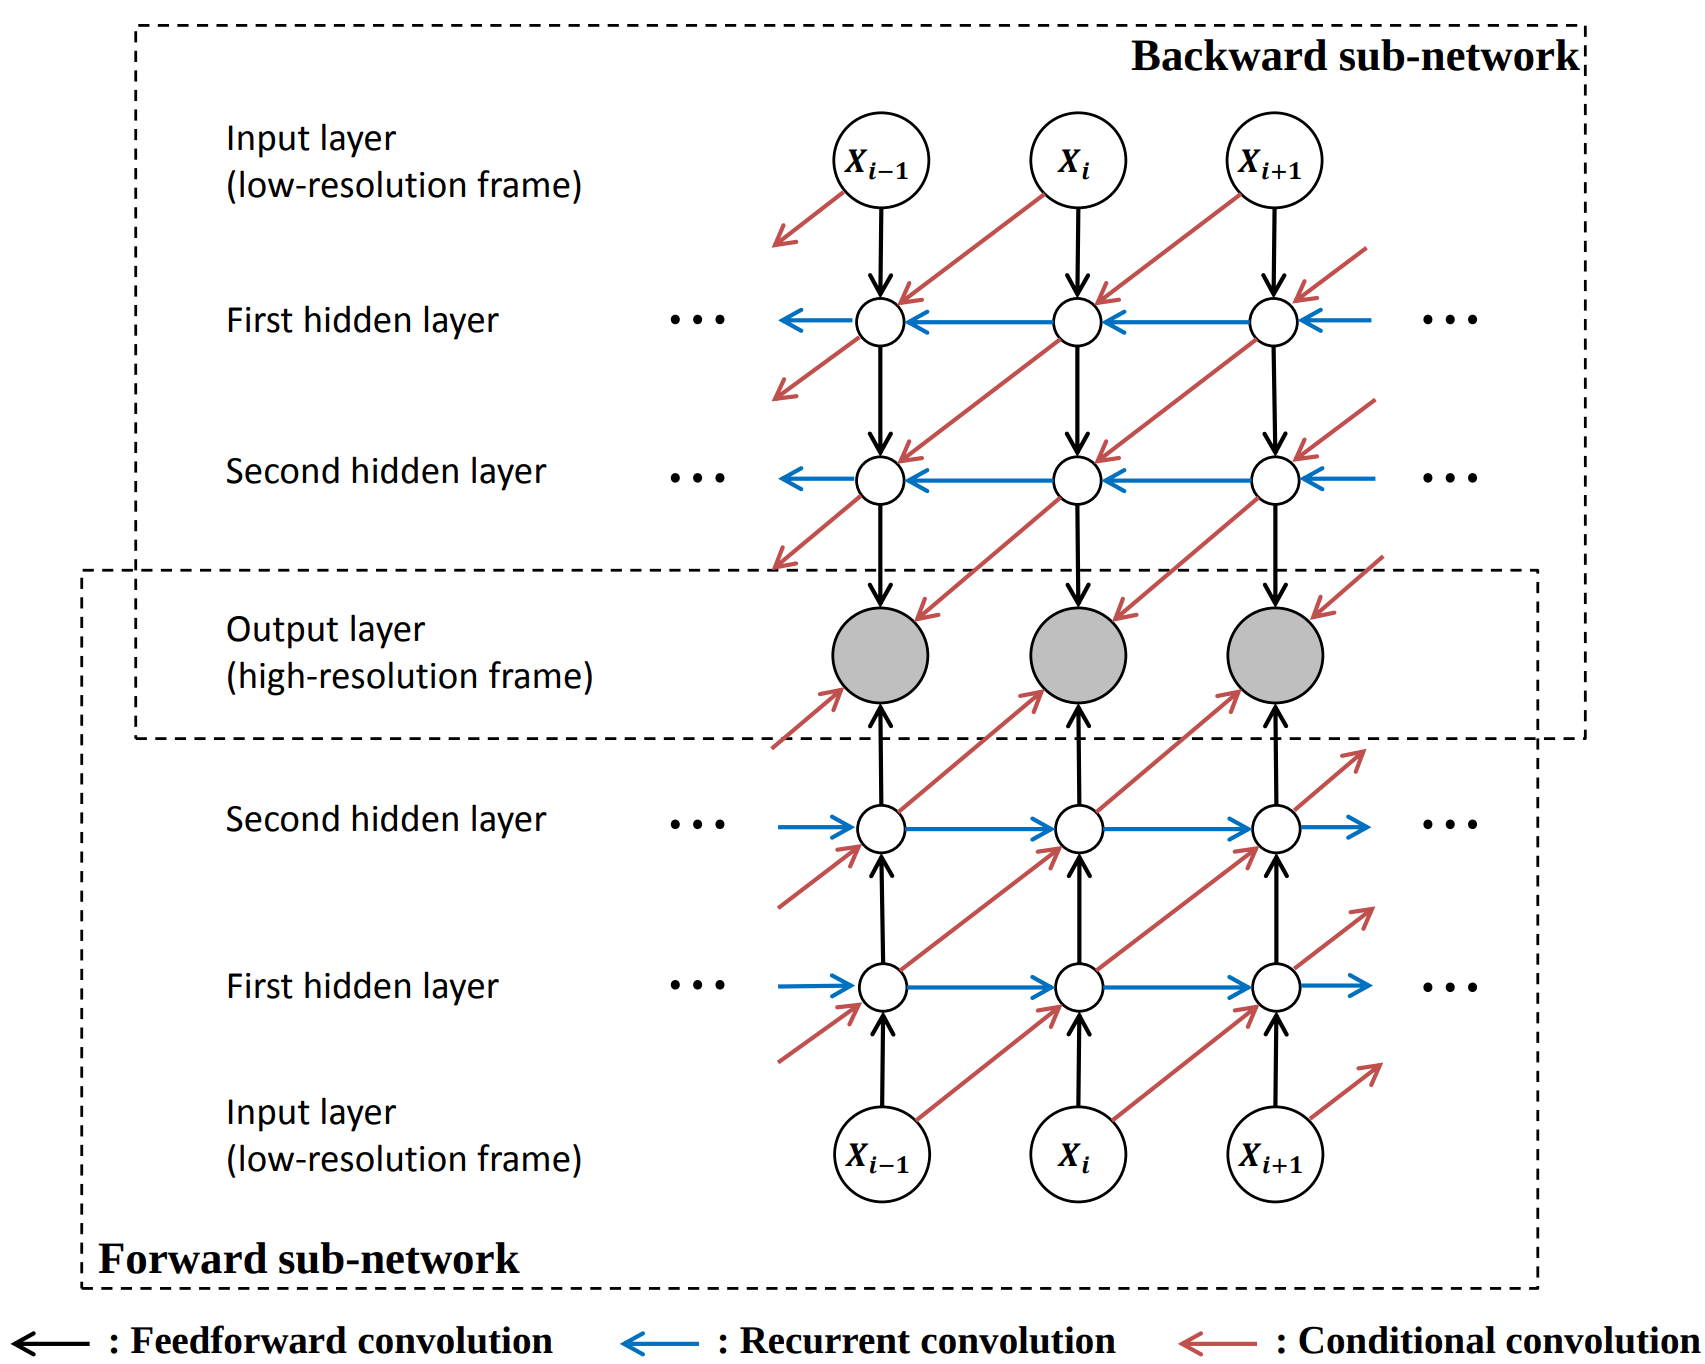
\includegraphics[width=.49\textwidth]{figures/neural_networks/brcn.png}
    \caption{BRCN schematic diagram\cite{huang2015bidirectional}.}\label{subfig:brcn}
\end{figure}
BRCN uses two recurrent networks, a forward-propagating network and a backward-propagating network.
%
Each of BRCN's RNNs is composed of conventional (feed-forward) convolutions, which model up-sampling, and convolutions in time (what they call recurrent and conditional convolutions), which model time dependencies (see figure~\ref{subfig:brcn}).
%
Note that the bi-directional framework incurs 3 image delay due the two hidden layers.
%
BRCN achieved (at the time) state of the art reconstruction performance for \(t=8\) image sequences but at \(\sim\)1s run-times it was far from real-time performance.
\subsubsection{Video Efficient Sub-Pixel Networks}
\begin{figure}
    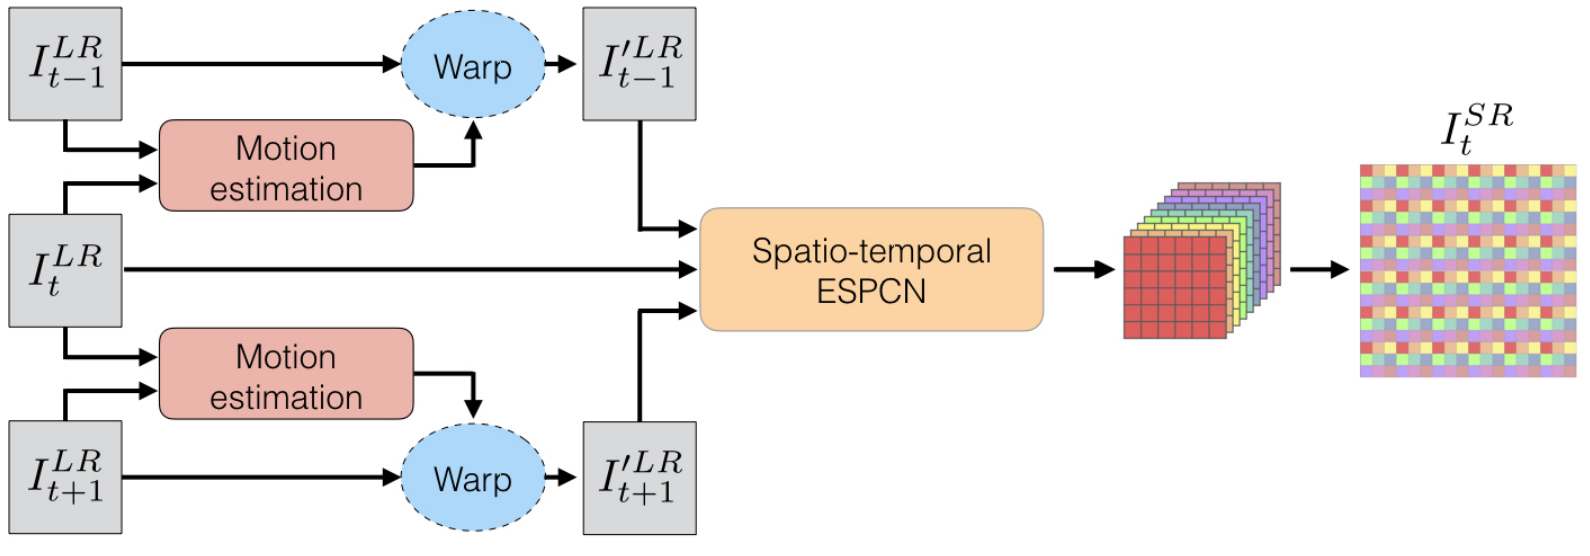
\includegraphics[width=.49\textwidth]{figures/neural_networks/realtime_epscn.png}
    \caption{Real-time MISR with motion compensation\cite{caballero2017real}.}\label{fig:realtimeepscn}
\end{figure}
The first real-time DNN architecture for MISR is based on efficient sub-pixel convolutions (see section~\ref{subsubsec:srgan}).
%
\begin{figure}
    \centering
    \newcommand*{\subfigwidth}{0.49\textwidth}
    \begin{subfigure}[b]{\subfigwidth}
        \centering
        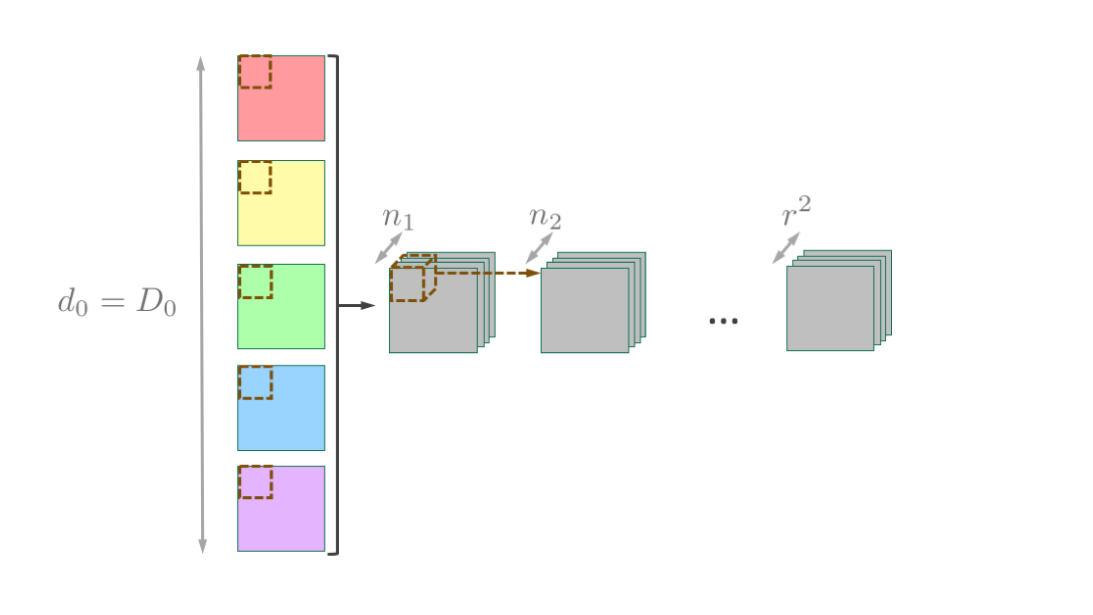
\includegraphics[width=.7\linewidth,keepaspectratio]{figures/neural_networks/early_fusion.png}
        \caption{Early fusion.}\label{subfig:earlyfus}
    \end{subfigure}
    \vskip\baselineskip
    \begin{subfigure}[b]{\subfigwidth}
        \centering
        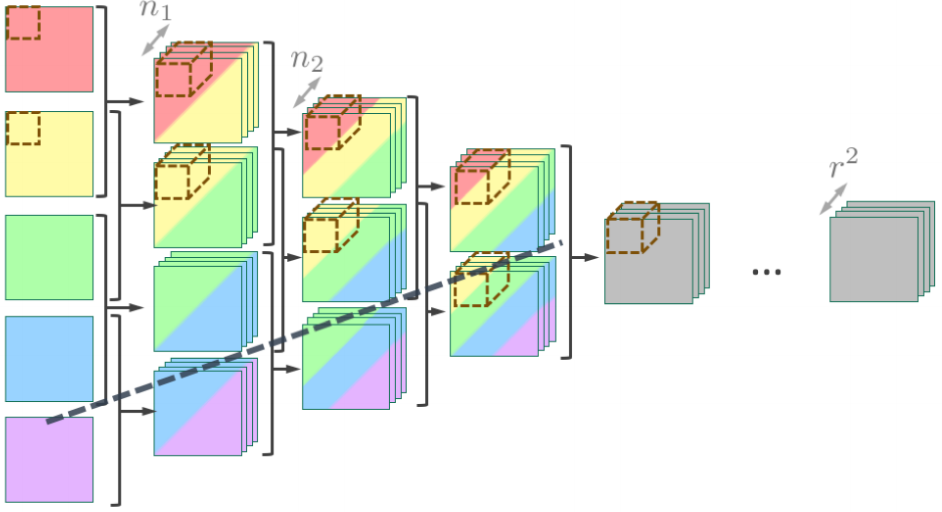
\includegraphics[width=\linewidth,keepaspectratio]{figures/neural_networks/slow_fusion.png}
        \caption{Slow fusion. If frames are processed in an online fashion then filter values should be shared. For example the last frame (purple) can recycle all of the computations above the dotted line.}\label{subfig:slowfus}
    \end{subfigure}
    % \vskip\baselineskip
    % \begin{subfigure}[b]{\subfigwidth}
    %     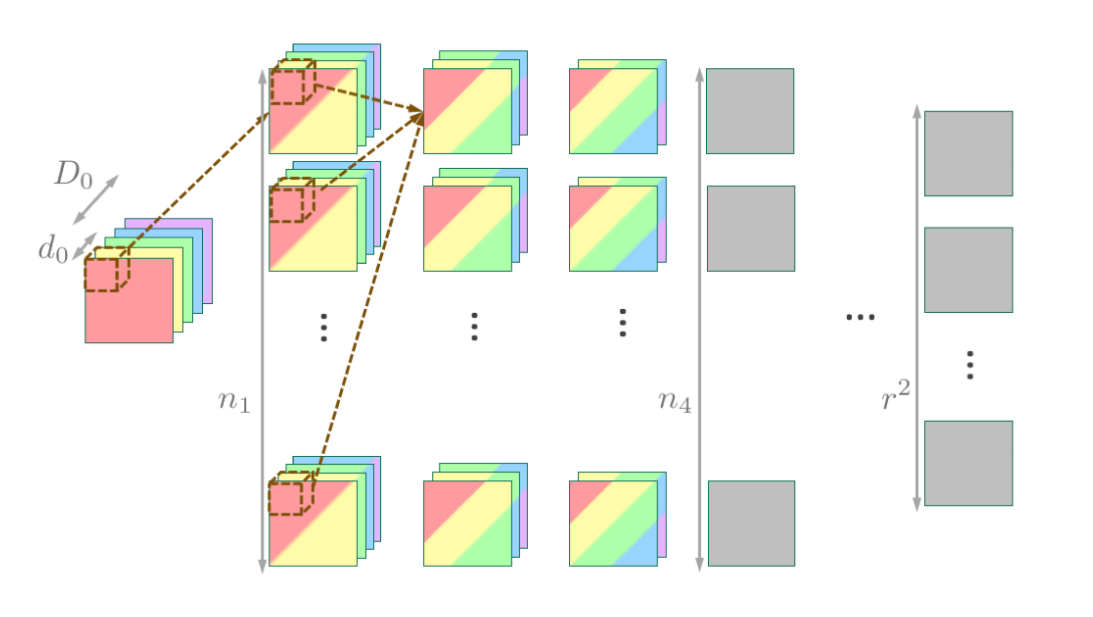
\includegraphics[width=\linewidth,keepaspectratio]{figures/neural_networks/3d_conv.png}
    %     \caption{3D convolution.}\label{subfig:updowndbpn}
    % \end{subfigure}
    \caption{Spatio-temporal ESPCN\cite{caballero2017real}.}\label{fig:fusions}
\end{figure}
Caballero \etal experiment with various \textit{fusion} methods for extracting non-redundant information from sequences of images.
%
Each fusion method applies convolutions to the sequence of images in either a tiered or conventional fashion (see figure~\ref{fig:fusions}).
%
Early fusion 
% \subsubsection{Temporally Coherent GAN}\label{subsubsec:tecogan}
% \subsubsection{Frame-Recurrent Video Super-Resolution}\label{subsubsec:frvsr}
% \subsubsection{Recurrent Back-Projection Network}\label{subsubsec:rbpn}
% \subsubsection{Enhanced Deformable Convolutional Networks}\label{subsubsec:edvr}
